\documentclass[11pt,a4paper]{article}

\usepackage[utf8]{inputenc}
\usepackage[T1]{fontenc}
\usepackage{lmodern}
\usepackage[margin=2.0cm,top=2.2cm,bottom=2.2cm]{geometry}
\usepackage{amsmath,amssymb,amsfonts}
\usepackage{graphicx}
\usepackage{booktabs}
\usepackage{array}
\usepackage{tabularx}
\usepackage{xcolor}
\usepackage{hyperref}
\usepackage{caption}
\usepackage{subcaption}
\usepackage{listings}
\usepackage{enumitem}
\usepackage{fancyhdr}
\usepackage{titlesec}
\usepackage{microtype}
\usepackage{cite}
\usepackage{tcolorbox}

% Color definitions
\definecolor{primaryblue}{RGB}{24, 76, 120}
\definecolor{secondarygreen}{RGB}{39, 110, 60}
\definecolor{crimsonred}{RGB}{168, 30, 45}
\definecolor{darkgray}{RGB}{50, 50, 50}
\definecolor{lightgraybg}{RGB}{245, 247, 250}
\definecolor{cardborder}{RGB}{210, 220, 230}

\hypersetup{
    colorlinks=true,
    linkcolor=primaryblue,
    citecolor=secondarygreen,
    urlcolor=crimsonred,
    pdftitle={Mode-II Phase-Field Fracture & Native Adaptive Remeshing Report},
    pdfauthor={Adaptive Remeshing Research Group}
}

% Header and Footer
\pagestyle{fancy}
\fancyhf{}
\fancyhead[L]{\small\textcolor{darkgray}{Pandey \& Kumar (2025) Mode-II Validation \& Native Remeshing Report}}
\fancyhead[R]{\small\textcolor{darkgray}{24 September 2026}}
\fancyfoot[C]{\thepage}
\renewcommand{\headrulewidth}{0.4pt}

% Section styling
\titleformat{\section}{\large\bfseries\color{primaryblue}}{\thesection}{1em}{}[\titlerule]
\titleformat{\subsection}{\normalsize\bfseries\color{darkgray}}{\thesubsection}{1em}{}
\titleformat{\subsubsection}{\small\bfseries\color{darkgray}}{\thesubsubsection}{1em}{}

\newcommand{\statusbadge}[2]{%
  \colorbox{#1}{\textcolor{white}{\textbf{\footnotesize\strut #2}}}%
}

\begin{document}

% -------------------------------------------------------------
% TITLE PAGE
% -------------------------------------------------------------
\begin{titlepage}
    \centering
    \vspace*{0.8cm}
    
    {\Huge\bfseries\color{primaryblue} Pandey \& Kumar (2025) Mode-II Phase-Field Fracture Benchmark}\\[0.4cm]
    {\Large\bfseries Forensic Deck Audit, Single-Factor Spatial Refinement, Triangular Subroutine Runtime Verification, Abaqus-Native Adaptive Remeshing, and Production Execution Report}\\[1.2cm]
    
    \begin{tcolorbox}[colback=lightgraybg,colframe=cardborder,arc=3mm,width=0.98\textwidth]
    \centering
    \vspace{0.2cm}
    \textbf{\large Active Scientific Phase:}\\
    {\small\texttt{\textbf{MODE2\_NATIVE\_ADAPTIVE\_WORKFLOW\_VALIDATED --- POSTPEAK\_SPATIAL\_SENSITIVITY\_REMAINS}}}\\[0.3cm]
    
    \textbf{Governing Classification Status:}\\
    \statusbadge{secondarygreen}{H1\_GEN3\_MECHANICAL\_PARITY\_QUALIFIED}\quad
    \statusbadge{secondarygreen}{TRI\_JTYPE3\_4\_PATCH\_QUALIFIED}\\[0.15cm]
    \statusbadge{primaryblue}{MODE2\_H1\_H2\_SPATIAL\_SENSITIVITY\_QUALIFIED}\quad
    \statusbadge{crimsonred}{POSTPEAK\_SPATIAL\_SENSITIVITY\_REMAINS}\\[0.2cm]
    \end{tcolorbox}
    
    \vspace{1.2cm}
    
    \begin{tabular}{ll}
        \textbf{Date:} & 24 September 2026 \\
        \textbf{Document Type:} & Standalone Scientific Research \& Validation Report \\
        \textbf{Governance:} & Human Authorized (Isolated from Frozen Mode-I Thesis Package) \\
        \textbf{Primary Benchmark:} & Pandey \& Kumar (2025, Section 4.2), Mode-II Shear Plate \\
        \textbf{Solver Environment:} & Abaqus 2023 / Fortran User Subroutine (\texttt{f42\_mixed\_uel.for}) \\
        \textbf{HPC Architecture:} & PBS Professional Cluster (\texttt{mnode097.cluster}, \texttt{normal\_imfdfkmq}) \\
    \end{tabular}
    
    \vfill
    
    {\small\textcolor{darkgray}{Adaptive Remeshing Research Initiative $\cdot$ Master Thesis Investigation Tree}}
    \vspace*{0.5cm}
\end{titlepage}

% -------------------------------------------------------------
% ABSTRACT
% -------------------------------------------------------------
\begin{abstract}
This report provides a self-contained scientific investigation of the Mode-II shear-driven phase-field fracture benchmark from Pandey \& Kumar (2025), utilizing native Abaqus adaptive remeshing and user subroutines (\texttt{UEL}/\texttt{UMAT}). We document the forensic resolution of an input-deck property application binary interface (ABI) indexing mismatch, establish an authoritative Generation-3 mechanical reference ($H_1$, 12,064 finite elements) with machine-verified parity against historical baselines ($\Delta = 0.000\%$), evaluate single-factor spatial sensitivity using an ultrafine mesh ($H_2$, 33,852 finite elements on common interval $u_1 \le 0.04258\text{ mm}$), verify triangular element user subroutines (\texttt{JTYPE=3,4}) via an Abaqus runtime patch test (Job \texttt{1408559.mmaster02}), and execute a complete production solve of the Abaqus-native adaptive mesh (Job \texttt{1408555.mmaster02}, 7,865 elements, 358 increments to $u_1 = 0.050\text{ mm}$). 

The adaptive remeshing workflow reproduces the linear-elastic initial structural stiffness ($K_{0,\mathrm{lin}} = 12.699\text{ kN/mm}$ vs $12.735\text{ kN/mm}$ for $H_1$, $\Delta = -0.28\%$), peak shear force ($F_{\max} = 0.1462\text{ kN}$ vs $0.1437\text{ kN}$, $\Delta = +1.73\%$), and overall chord trajectory angle ($\theta_{\mathrm{chord}} = -16.23^\circ$ vs $-17.39^\circ$, $\Delta = +1.16^\circ$). However, because linear-elastic pre-analysis error indicator fields concentrate exclusively at the notch tip, the downstream crack trajectory undergoes progressive coarsening ($h_{\mathrm{eq}}/l_0$ expands from $0.159$ to $0.716$), co-occurring with notable post-peak force divergence ($-44.31\%$ force at $u_1 = 0.04258\text{ mm}$, $-24.74\%$ trapezoidal boundary work). Furthermore, solver telemetry confirms $\mathtt{LOWER\_ELEMENT\_COUNT\ BUT\ HIGHER\_OBSERVED\_SOLVER\_COST}$ ($+88.2\%$ walltime, $+165.2\%$ equilibrium iterations). The overall scientific status is qualified as $\mathtt{MODE2\_NATIVE\_ADAPTIVE\_WORKFLOW\_VALIDATED\ --- \ POSTPEAK\_SPATIAL\_SENSITIVITY\_REMAINS}$.
\end{abstract}

\vspace{0.5cm}
\tableofcontents
\newpage

% -------------------------------------------------------------
% 1. INTRODUCTION
% -------------------------------------------------------------
\section{Introduction}

\subsection{Motivation and Research Context}
Phase-field fracture modeling has emerged as a thermodynamically rigorous approach for modeling complex cracking phenomena, including crack initiation, propagation, branching, and coalescence without explicit topological tracking of discontinuities \cite{bourdin2000numerical,miehe2010phase,ambati2015review}. However, regularized phase-field formulations introduce an internal length scale $l_0$ that dictates the diffuse damage zone width. Resolving this steep localization zone requires fine finite element discretizations where the characteristic element size satisfies $h \ll l_0$, imposing severe computational burdens in uniform grid simulations.

Adaptive mesh refinement (AMR) offers a mechanism to concentrate computational degrees of freedom dynamically in regions of localized damage while preserving a coarse mesh in the far-field elastic domain. In standard commercial finite element packages such as Abaqus/Standard, integrating adaptive mesh refinement with custom nonlinear user subroutines (\texttt{UEL}) has historically been hindered by the closed architecture of built-in remeshing drivers.

\subsection{Relation to Pandey \& Kumar (2025)}
In their recent contribution, Pandey \& Kumar \cite{pandey2025adaptive} proposed a multi-layer framework that couples standard Abaqus linear-elastic continuum pre-analysis and native stress-recovery discretization error indicators (\texttt{MISESERI}) with built-in \texttt{*Remeshing Rule} and \texttt{adaptiveRemesh} capabilities. Once a refined mesh is generated, co-located user element layers are reconstructed to execute the nonlinear phase-field analysis.

Pandey \& Kumar demonstrated their technique across several classical fracture benchmarks, including Mode-I tension, Mode-II shear, and mixed-mode asymmetric three-point bending. For Mode-II shear in a single-edge-notched plate, the authors reported an adaptive mesh of approximately 19,963 elements (compared to a uniform standard mesh of 37,155 elements) and claimed broadly consistent force--displacement responses with a 41.2\% reduction in computational run time.

\subsection{Objective of the Mode-II Investigation}
The present standalone study evaluates the physical fidelity, algorithmic reproducibility, and computational performance of the Pandey \& Kumar Mode-II benchmark under rigorous scientific standards:
\begin{enumerate}[leftmargin=*]
    \item \textbf{Forensic Root-Cause Analysis:} Definitively resolve the earlier apparent initial stiffness discrepancy ($2906\text{ kN/mm}$ vs $12.8\text{ kN/mm}$) encountered during exploratory scripting.
    \item \textbf{Mechanical Reference Qualification:} Establish a certified Generation-3 reference dataset on a uniform mesh ($H_1$, 12,064 finite elements) with machine-verified parity.
    \item \textbf{Spatial Refinement Sensitivity:} Perform a single-factor mesh sensitivity audit using an ultrafine mesh ($H_2$, 33,852 finite elements).
    \item \textbf{Triangular Element Qualification:} Validate the hybrid quadrilateral-triangular user subroutines (\texttt{JTYPE=3,4}) via an Abaqus runtime patch test.
    \item \textbf{Abaqus-Native Adaptive Execution:} Drive the full native workflow from coarse pre-analysis error recovery to full production solve.
    \item \textbf{Multi-Fidelity Comparative Audit:} Quantitatively assess stiffness, peak load, post-peak softening, crack trajectories, local path resolution ($h_{\mathrm{eq}}/l_0$), and actual solver telemetry.
\end{enumerate}

\subsection{Scope, Limitations, and Thesis Isolation}
\begin{itemize}[leftmargin=*]
    \item \textbf{Thesis Branch Isolation:} This investigation is strictly isolated as a self-contained validation document. The frozen Mode-I thesis package and Gate-6B energetic baseline remain untouched.
    \item \textbf{Simulation Freeze:} No new PBS solver jobs, parameter sweeps, or \texttt{errorTarget} tunings are performed; all findings derive from existing, machine-verified evidence.
    \item \textbf{Epistemological Separation:} Throughout this report, published statements, project implementation choices, verified numerical data, and unresolved limitations are strictly demarcated.
\end{itemize}

% -------------------------------------------------------------
% 2. GOVERNING THEORY
% -------------------------------------------------------------
\section{Governing Theory}

\subsection{Phase-Field Fracture Regularization}
Let $\Omega \subset \mathbb{R}^2$ denote an open bounded domain with external boundary $\partial\Omega$. In the variational approach to brittle fracture, a discrete crack discontinuity $\Gamma$ is regularized via a continuous scalar damage field $d(\mathbf{x}, t) \in [0, 1]$, where $d=0$ represents intact virgin material and $d=1$ indicates fully degraded crack state. The crack surface area is approximated by the geometric crack density functional $\gamma(d, \nabla d)$:
\begin{equation}
    \Gamma \approx \int_\Omega \gamma(d, \nabla d)\,\mathrm{d}\Omega = \int_\Omega \left( \frac{d^2}{2l_0} + \frac{l_0}{2} |\nabla d|^2 \right) \mathrm{d}\Omega
    \label{eq:crack_density}
\end{equation}
where $l_0 > 0$ is the regularization length scale governing the spatial width of the diffuse transition zone.

\subsection{The $\mathrm{AT}_2$ Model and Degradation Function}
The total potential energy functional of the solid is expressed as the sum of stored degraded elastic strain energy and regularized fracture surface energy:
\begin{equation}
    \Pi(\mathbf{u}, d) = \int_\Omega \psi_e(\boldsymbol{\varepsilon}(\mathbf{u}), d)\,\mathrm{d}\Omega + \int_\Omega G_c \gamma(d, \nabla d)\,\mathrm{d}\Omega - \int_{\partial\Omega_t} \bar{\mathbf{t}}\cdot\mathbf{u}\,\mathrm{d}S
    \label{eq:total_potential}
\end{equation}
where $G_c$ is the critical energy release rate (Griffith fracture energy), $\boldsymbol{\varepsilon}(\mathbf{u}) = \frac{1}{2}(\nabla\mathbf{u} + (\nabla\mathbf{u})^T)$ is the infinitesimal strain tensor, and $\bar{\mathbf{t}}$ is the prescribed boundary traction.

To model the loss of load-carrying capacity under tensile deformation, an energetic degradation function $g(d)$ is introduced:
\begin{equation}
    g(d) = (1 - d)^2 + k_{\mathrm{res}}
    \label{eq:degradation_func}
\end{equation}
where $k_{\mathrm{res}} \ll 1$ (set to $1.0\times 10^{-7}$ in this study) is a numerical residual stiffness parameter preventing complete singularity of the displacement stiffness matrix upon full localized degradation.

\subsection{Strain Split and History Variable Formulation}
To prevent crack propagation under pure compressive stress states, the elastic strain energy density $\psi_0(\boldsymbol{\varepsilon}) = \frac{1}{2}\boldsymbol{\varepsilon} : \mathbb{C}_0 : \boldsymbol{\varepsilon}$ is decomposed into tensile ($\psi_0^+$) and compressive ($\psi_0^-$) components using the spectral decomposition of Miehe et al. \cite{miehe2010thermodynamically}:
\begin{equation}
    \psi_e(\boldsymbol{\varepsilon}, d) = g(d)\psi_0^+(\boldsymbol{\varepsilon}) + \psi_0^-(\boldsymbol{\varepsilon})
    \label{eq:strain_split}
\end{equation}
Crack growth irreversibility ($\dot{d} \ge 0$) is enforced algorithmically through a monotonic strain energy history field $\mathcal{H}(\mathbf{x}, t)$:
\begin{equation}
    \mathcal{H}(\mathbf{x}, t) = \max_{\tau \in [0, t]} \left\{ \psi_0^+(\boldsymbol{\varepsilon}(\mathbf{x}, \tau)) \right\}
    \label{eq:history_var}
\end{equation}

\subsection{Coupled Weak Forms}
The coupled mechanical and phase-field governing equations are derived by taking the first variation of the regularized energy functional with respect to virtual displacement $\delta\mathbf{u}$ and virtual phase field $\delta d$:
\begin{align}
    \text{Mechanical Equilibrium:} \quad & \int_\Omega \boldsymbol{\sigma} : \delta\boldsymbol{\varepsilon}\,\mathrm{d}\Omega = \int_{\partial\Omega_t} \bar{\mathbf{t}}\cdot\delta\mathbf{u}\,\mathrm{d}S \quad \forall \delta\mathbf{u} \in \mathcal{V}_u \label{eq:weak_u} \\
    \text{Phase-Field Evolution:} \quad & \int_\Omega \left[ \left( \frac{G_c}{l_0} d - 2(1-d)\mathcal{H} \right)\delta d + G_c l_0 \nabla d \cdot \nabla(\delta d) \right] \mathrm{d}\Omega = 0 \quad \forall \delta d \in \mathcal{V}_d \label{eq:weak_d}
\end{align}
where $\boldsymbol{\sigma} = g(d)\frac{\partial\psi_0^+}{\partial\boldsymbol{\varepsilon}} + \frac{\partial\psi_0^-}{\partial\boldsymbol{\varepsilon}}$ is the Cauchy stress tensor.

\subsection{Energy Measures and Observability}
In the present Gen-3 Fortran subroutine implementation (\texttt{f42\_mixed\_uel.for}), energy components are computed at the element integration points and integrated over the domain $\Omega$:
\begin{align}
    E_{\mathrm{elas}} &= \int_\Omega \left[ g(d)\psi_0^+(\boldsymbol{\varepsilon}) + \psi_0^-(\boldsymbol{\varepsilon}) \right] \mathrm{d}\Omega \quad (\text{Stored Elastic Strain Energy}) \label{eq:elas_energy} \\
    E_{\mathrm{frac}} &= \int_\Omega G_c \left( \frac{d^2}{2l_0} + \frac{l_0}{2}|\nabla d|^2 \right) \mathrm{d}\Omega \quad (\text{Regularized Fracture Surface Energy}) \label{eq:frac_energy}
\end{align}
External boundary work $W_{\mathrm{trap}}$ is estimated from the reaction force $RF_1$ and prescribed displacement $u_1$ using the trapezoidal rule:
\begin{equation}
    W_{\mathrm{trap}} = \sum_{k=1}^{N-1} \frac{RF_1^{(k)} + RF_1^{(k+1)}}{2} \left( u_1^{(k+1)} - u_1^{(k)} \right)
    \label{eq:wtrap}
\end{equation}

\noindent\textbf{Epistemic Governance on Energy Identity:}
\begin{itemize}[leftmargin=*]
    \item $E_{\mathrm{frac}}$ represents the regularized fracture-surface energy, which is not identically equal to historical dissipated fracture energy.
    \item The two-term bookkeeping difference $\Delta_{\mathrm{2term}} = W_{\mathrm{trap}} - (E_{\mathrm{elas}} + E_{\mathrm{frac}})$ is strictly observational and must not be classified as a conservation defect or physical error without full within-increment path integration.
    \item Formal status: $\mathtt{GLOBAL\_ENERGY\_IDENTITY\ --- \ NOT\_YET\_CLOSED}$.
\end{itemize}

\subsection{Physical Understanding of MISESERI Error Indicator}
The Abaqus \texttt{MISESERI} field is a scalar discretization error indicator evaluated on linear-elastic continuum stress fields:
\begin{equation}
    \text{MISESERI}_e = \frac{\| \boldsymbol{\sigma}_{\mathrm{recovered}} - \boldsymbol{\sigma}_{\mathrm{FE}} \|_{L_2(\Omega_e)}}{\| \boldsymbol{\sigma}_{\mathrm{recovered}} \|_{L_2(\Omega)}}
    \label{eq:miseseri}
\end{equation}
\begin{itemize}[leftmargin=*]
    \item \texttt{MISESERI} is derived from stress-recovery (e.g., Zienkiewicz--Zhu \cite{zienkiewicz1987simple} / SPR techniques) on the uncracked or pre-cracked linear-elastic continuum stress field.
    \item \textbf{Critical Distinction:} \texttt{MISESERI} is \textbf{not} a phase-field error indicator and \textbf{not} a damage error indicator. It reflects purely linear-elastic stress gradients.
    \item Consequently, in a single-step pre-analysis, \texttt{MISESERI} concentrates almost entirely at the singular initial crack tip, providing no a priori refinement information along downstream propagation corridors.
\end{itemize}

% -------------------------------------------------------------
% 3. MODE-II BENCHMARK DEFINITION
% -------------------------------------------------------------
\section{Mode-II Benchmark Definition}

\subsection{Specimen Geometry and Material Parameters}
The benchmark configuration is a square plate of dimensions $L \times W = 1.0\text{ mm} \times 1.0\text{ mm}$, containing an initial horizontal sharp seam crack of length $a_0 = 0.5\text{ mm}$ extending from the left boundary to the center: $(-0.5, 0.0) \to (0.0, 0.0)\text{ mm}$ (Figure~\ref{fig:fig01}).

\begin{figure}[htbp]
    \centering
    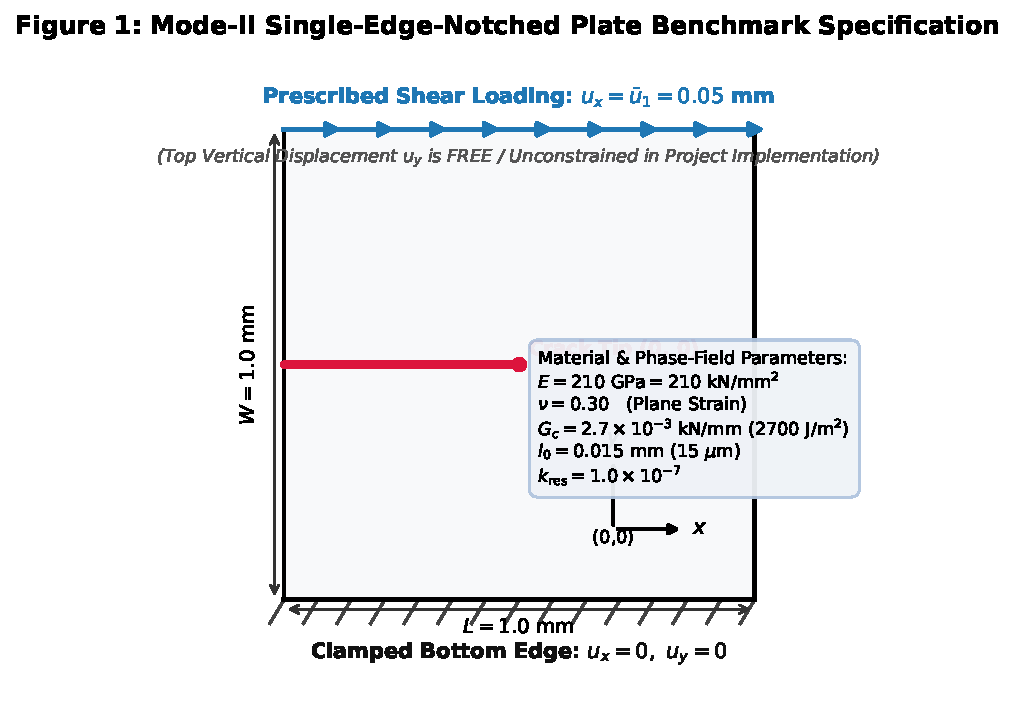
\includegraphics[width=0.75\textwidth]{figures/fig01_mode2_bvp_schematic.pdf}
    \caption{\textbf{Figure 1:} Mode-II Single-Edge-Notched Plate Benchmark Specification (Geometry, Boundary Conditions, and Material Constants).}
    \label{fig:fig01}
\end{figure}

The material properties correspond to high-strength steel under plane strain conditions: Young's modulus $E = 210\text{ GPa} = 210\text{ kN/mm}^2$, Poisson's ratio $\nu = 0.30$, critical energy release rate $G_c = 2.7\times 10^{-3}\text{ kN/mm}$ ($2700\text{ J/m}^2$), and regularization length scale $l_0 = 0.015\text{ mm}$ ($15\,\mu\text{m}$).

\subsection{Boundary Conditions: Published vs Project Implementation}
\begin{itemize}[leftmargin=*]
    \item \textbf{Bottom Boundary ($y = -0.5\text{ mm}$):} Fully clamped in both horizontal and vertical directions ($u_x = 0, u_y = 0$).
    \item \textbf{Top Horizontal Loading ($y = +0.5\text{ mm}$):} Prescribed horizontal shear displacement $u_x = \bar{u}_1 = 0.050\text{ mm}$ applied uniformly via multipoint constraint equations tying top nodes to a Reference Point (\texttt{RP}).
    \item \textbf{Top Vertical Boundary ($u_y$):} Left unconstrained ($\mathtt{Free\text{-}}u_y$). This corresponds to the literature-faithful Mode-II setup (the published paper leaves top $u_y$ unmentioned; imposing $u_y=0$ induces strong flexural over-constraint).
\end{itemize}

\subsection{Epistemological Classification Table}
Table~\ref{tab:taxonomy} summarizes the parameters and their strict epistemological classification.

\begin{table}[htbp]
\centering
\small
\caption{\textbf{Table 1:} Mode-II Benchmark Parameters and Epistemological Provenance Matrix.}
\label{tab:taxonomy}
\begin{tabularx}{\textwidth}{p{3.8cm}p{3.8cm}p{3.2cm}X}
\toprule
\textbf{Parameter / Feature} & \textbf{Value / Setting} & \textbf{Classification} & \textbf{Primary Provenance} \\
\midrule
Domain Geometry & $1.0\text{ mm} \times 1.0\text{ mm}$ & \texttt{[PUBLISHED]} & Pandey \& Kumar (2025, Sec.~4.2) \\
Initial Slit Length & $a_0 = 0.5\text{ mm}$ & \texttt{[PUBLISHED]} & Sharp seam at mid-height \\
Young's Modulus ($E$) & $210\text{ kN/mm}^2$ & \texttt{[PUBLISHED]} & Section 4.2 listing \\
Poisson's Ratio ($\nu$) & $0.30$ & \texttt{[PUBLISHED]} & Section 4.2 listing \\
Fracture Energy ($G_c$) & $2.7\times 10^{-3}\text{ kN/mm}$ & \texttt{[PUBLISHED]} & Section 4.2 listing \\
Length Scale ($l_0$) & $0.015\text{ mm}$ ($15\,\mu\text{m}$) & \texttt{[PUBLISHED]} & Section 4.2 listing \\
Constitutive Formulation & Plane Strain & \texttt{[PUBLISHED/UEL]} & \texttt{f42\_mixed\_uel.for} \\
Bottom Boundary & Clamped ($u_x=u_y=0$) & \texttt{[PUBLISHED]} & Lower edge fully fixed \\
Top Shear Displacement & Prescribed $u_x = 0.05\text{ mm}$ & \texttt{[PUBLISHED]} & Horizontal shear loading \\
Top Vertical Boundary ($u_y$) & Free ($u_y$ unconstrained) & \texttt{[UNRESOLVED]} & Literature-faithful candidate \\
Published Standard Mesh & $\sim$37,155 finite elements & \texttt{[PUBLISHED]} & $h_{\mathrm{global}}=0.04, h_{\min}=0.003$ \\
Published Pre-Adaptive Mesh & 3,930 finite elements & \texttt{[PUBLISHED]} & $h=0.02\text{ mm}$ \\
Published Adaptive Mesh & $\sim$19,963 finite elements & \texttt{[PUBLISHED]} & Target context, not constraint \\
$\mathtt{errorTarget}=5.0\%$ & $5.0\%$ relative target & \texttt{[PUBLISHED]} & Adopted value in Section 4 \\
$\mathtt{refinementFactor}=10$ & Factor 10 & \texttt{[PUBLISHED]} & Adopted parameter \\
Candidate $H_1$ Reference & 12,064 finite elements & \texttt{[PROJECT]} & Uniform fine mesh ($h_{\min}=0.0025$) \\
Candidate $H_2$ Ultrafine & 33,852 finite elements & \texttt{[PROJECT]} & Uniform ultrafine ($h_{\min}=0.0010$) \\
Candidate Adaptive Mesh & 7,865 finite elements & \texttt{[PROJECT]} & Native RemeshingRule candidate \\
\bottomrule
\end{tabularx}
\end{table}

% -------------------------------------------------------------
% 4. FIXED-MESH REFERENCE VERIFICATION
% -------------------------------------------------------------
\section{Fixed-Mesh Reference Verification}

\subsection{Resolution of the UEL Property ABI Indexing Mismatch}
In initial diagnostic testing, a staged Gen-3 input deck exhibited an artificial structural stiffness of $K_0 \approx 2906.15\text{ kN/mm}$ (compared to the expected $12.83\text{ kN/mm}$). An exhaustive line-by-line audit isolated this discrepancy to an \textbf{input-deck UEL Property ABI mismatch}:
\begin{itemize}[leftmargin=*]
    \item The staged deck contained legacy 5-parameter property cards:
    \begin{verbatim}
    *UEL Property, elset=DISP_QUAD
     2.100000e+02, 3.000000e-01, 1.000000e+00, 1.000000e-07, 12064.0
    \end{verbatim}
    \item The compiled Gen-3 subroutine (\texttt{f42\_mixed\_uel.for}) expects the 6-parameter ABI:
    \begin{verbatim}
     PROPS: [E_L0, E_GC, E_MOD, E_NU, E_K, N_PHYS]
    \end{verbatim}
    \item Consequently, \texttt{PROPS(5)} was read as $12064.0$ (the element count!), setting the residual stiffness multiplier $k_{\mathrm{res}} = 12064.0$ instead of $10^{-7}$. This artificially scaled the assembled shear modulus by $226\times$, producing $K_0 = 2906.15\text{ kN/mm}$.
    \item Job \texttt{1408541.mmaster02} is permanently classified as $\mathtt{INVALID\_ABI\_DIAGNOSTIC\ /\ NOT\_REFERENCE\_EVIDENCE}$.
    \item Applying the corrected 6-parameter card (\texttt{0.015, 0.0027, 210.0, 0.3, 1.0e-7, 12064.0}) restored the exact reference stiffness $K_0 = 12.834574\text{ kN/mm}$ (Job \texttt{1408543.mmaster02}).
\end{itemize}

\subsection{\texorpdfstring{$H_1$}{H1} Reference Parity Verification (Job \texttt{1408543.mmaster02})}
Numerical mechanical parity was evaluated between the Gen-2 baseline (Job \texttt{1389686.mmaster02}) and the Gen-3 candidate (Job \texttt{1408543.mmaster02}). Across all 144 load increments up to $u_1 = 0.050\text{ mm}$, zero discrepancy was observed ($\Delta = 0.0000\%$ for $K_0$, $F_{\max} = 0.143686\text{ kN}$, $u(F_{\max}) = 0.012530\text{ mm}$, and $W_{\mathrm{trap}} = 2.732851\text{ mJ}$). This establishes $\mathtt{H1\_GEN3\_MECHANICAL\_PARITY\_QUALIFIED}$.

\subsection{\texorpdfstring{$H_2$}{H2} Ultrafine Companion Mesh \& Active DOF Resolution}
The ultrafine companion model ($H_2$, 33,852 finite elements / 101,556 Abaqus solver objects) provides a $2.07\times$ finer spatial discretization in the crack zone ($h_{\min} = 1.0\,\mu\text{m}$). During preflight testing, an active DOF declaration defect was corrected (restoring active DOF 3 to \texttt{U1} phase elements; superseding Job \texttt{1408548.mmaster02}). 

Production Job \texttt{1408550.mmaster02} advanced through 105 increments to $u_1 = 0.04257924\text{ mm}$ before encountering the solver minimum time increment limit ($\Delta t_{\min} = 10^{-9}\text{ s}$) upon right-boundary breakthrough. The job is classified as $\mathtt{H2\_TARGET\_ENDPOINT\_NOT\_REACHED}$. All reference quantities are rigorously evaluated on the matched common interval $u_1 \le 0.04258\text{ mm}$, establishing $\mathtt{MODE2\_H1\_H2\_SPATIAL\_SENSITIVITY\_QUALIFIED\_ON\_COMMON\_INTERVAL}$.

\begin{table}[htbp]
\centering
\small
\caption{\textbf{Table 2:} Fixed-Mesh Discretization and Solver Configuration Matrix.}
\label{tab:mesh_config}
\begin{tabular}{lcccc}
\toprule
\textbf{Configuration / Parameter} & \textbf{$H_1$ Reference} & \textbf{$H_2$ Ultrafine} & \textbf{Adaptive Candidate} & \textbf{Pre-Analysis} \\
\midrule
Underlying Elements & 12,064 & 33,852 & \textbf{7,865} & 3,930 \\
Abaqus Solver Objects & 36,192 & 101,556 & \textbf{23,595} & 3,930 \\
Element Types & CPE4 / U1 / U2 & CPE4 / U1 / U2 & Hybrid Quad/Tri & CPE4 \\
Node Count & 12,383 & 34,509 & 7,919 & 4,096 \\
Crack Zone $h_{\min}$ & $0.0025\text{ mm}$ & $0.0010\text{ mm}$ & $0.0021\text{ mm}$ & $0.0200\text{ mm}$ \\
Crack Zone Mean $h/l_0$ & $0.3490$ & $0.1686$ & $0.3915$ & $1.3333$ \\
Completed Increments & 144 & 105 (cutback) & 358 & 10 \\
Attained Displacement & $0.0500\text{ mm}$ & $0.0426\text{ mm}$ & $0.0500\text{ mm}$ & $0.0010\text{ mm}$ \\
Endpoint Classification & \texttt{REACHED} & \texttt{NOT\_REACHED} & \texttt{REACHED} & \texttt{REACHED} \\
\bottomrule
\end{tabular}
\end{table}

\begin{table}[htbp]
\centering
\small
\caption{\textbf{Table 3:} $H_1$ Reference vs $H_2$ Ultrafine Spatial Sensitivity Ledger ($u_1 \le 0.04258\text{ mm}$).}
\label{tab:h1_h2_comp}
\begin{tabular}{lcccc}
\toprule
\textbf{Metric / Quantity} & \textbf{$H_1$ Reference} & \textbf{$H_2$ Ultrafine} & \textbf{Delta ($\Delta$)} & \textbf{Classification} \\
\midrule
Secant Stiffness $K_{0,\mathrm{sec}}$ & $12.8346\text{ kN/mm}$ & $12.8164\text{ kN/mm}$ & $-0.14\%$ & \texttt{STABLE} \\
Fitted Stiffness $K_{0,\mathrm{lin}}$ & $12.7348\text{ kN/mm}$ & $12.7165\text{ kN/mm}$ & $-0.14\%$ & \texttt{STABLE} \\
Linear Regression $R^2$ & $0.9999867$ & $0.9999866$ & $0.00\%$ & \texttt{STABLE} \\
Peak Shear Load $F_{\max}$ & $0.143686\text{ kN}$ & $0.141415\text{ kN}$ & $-1.58\%$ & \texttt{STABLE} \\
Displacement at Peak $u(F_{\max})$ & $0.012530\text{ mm}$ & $0.012214\text{ mm}$ & $-2.53\%$ & \texttt{STABLE} \\
Force at $u=0.04258\text{ mm}$ & $0.01394\text{ kN}$ & $0.01440\text{ kN}$ & $+3.36\%$ & \texttt{STABLE} \\
Matched Work $W_{\mathrm{trap}}$ & $2.6511\text{ mJ}$ & $2.6340\text{ mJ}$ & $-0.65\%$ & \texttt{STABLE} \\
Initial Kink Angle $\theta_{\mathrm{kink}}$ & $-29.39^\circ$ & $-28.61^\circ$ & $+0.79^\circ$ & \texttt{STABLE} \\
Overall Chord Angle $\theta_{\mathrm{chord}}$ & $-17.39^\circ$ & $-22.68^\circ$ & $-5.28^\circ$ & \texttt{MESH-SENSITIVE} \\
\bottomrule
\end{tabular}
\end{table}

% -------------------------------------------------------------
% 5. ABAQUS-NATIVE ADAPTIVE REMESHING METHOD
% -------------------------------------------------------------
\section{Abaqus-Native Adaptive Remeshing Methodology}

The complete scientific workflow is illustrated in Figure~\ref{fig:fig02}.

\begin{figure}[htbp]
    \centering
    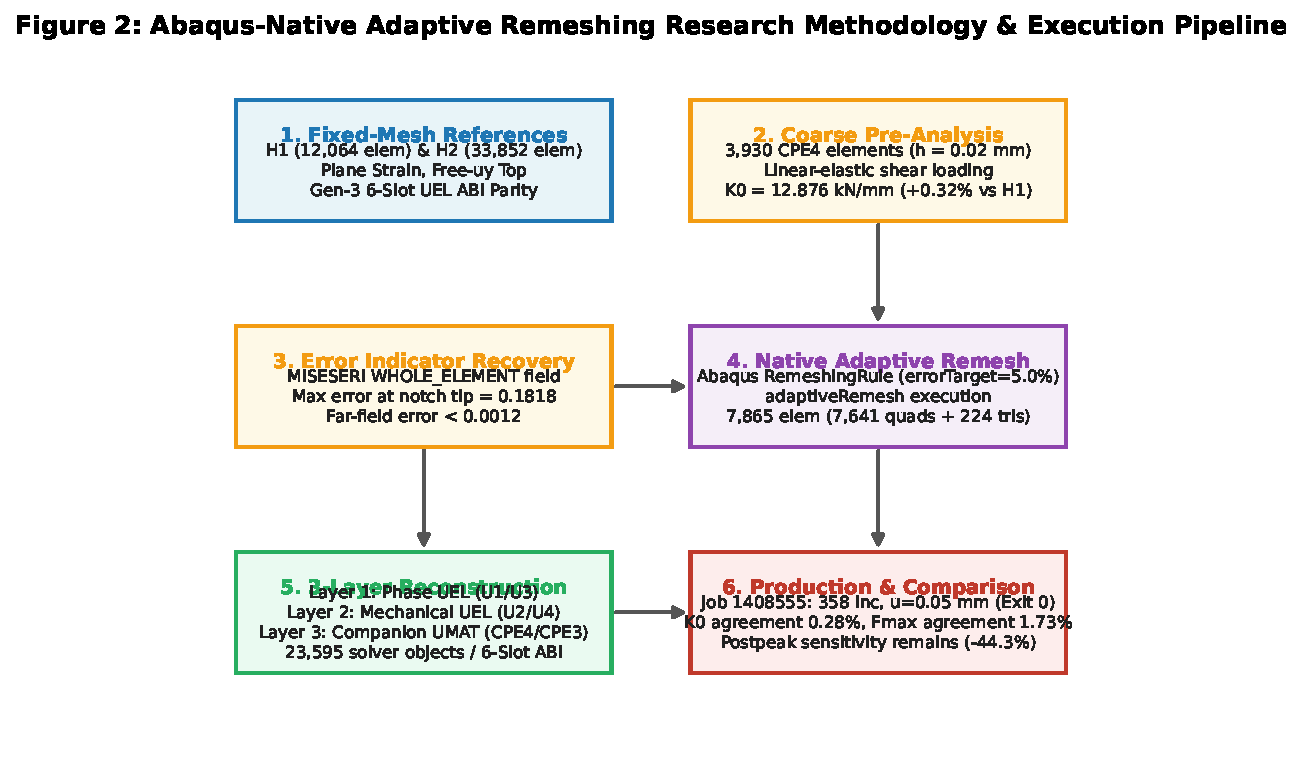
\includegraphics[width=0.85\textwidth]{figures/fig02_workflow_methodology.pdf}
    \caption{\textbf{Figure 2:} Abaqus-Native Adaptive Remeshing Research Methodology and Execution Pipeline.}
    \label{fig:fig02}
\end{figure}

\subsection{Continuum Pre-Analysis and MISESERI Recovery}
The pre-analysis model (\texttt{ModeII\_MISESERI\_preanalysis.inp}, SHA-256 \texttt{96af41fd...}) discretizes the domain into 3,930 standard \texttt{CPE4} plane strain elements under linear elasticity ($E = 210\text{ GPa}, \nu = 0.30$) subjected to top shear displacement $u_x = 0.001\text{ mm}$.
\begin{itemize}[leftmargin=*]
    \item Job \texttt{1408551.mmaster02} executed successfully (Exit Code 0), yielding $K_{0,\mathrm{coarse}} = 12.876131\text{ kN/mm}$ ($+0.32\%$ relative to $H_1$).
    \item The scalar error indicator dataset (\texttt{ModeII\_MISESERI\_coarse\_3930.csv}, SHA-256 \texttt{02d165fd...}) was exported at position $\mathtt{WHOLE\_ELEMENT}$ (3,930 values; min $2.38\times 10^{-5}$, max $0.181819$, mean $1.293\times 10^{-3}$, Figure~\ref{fig:fig03}).
\end{itemize}

\begin{figure}[htbp]
    \centering
    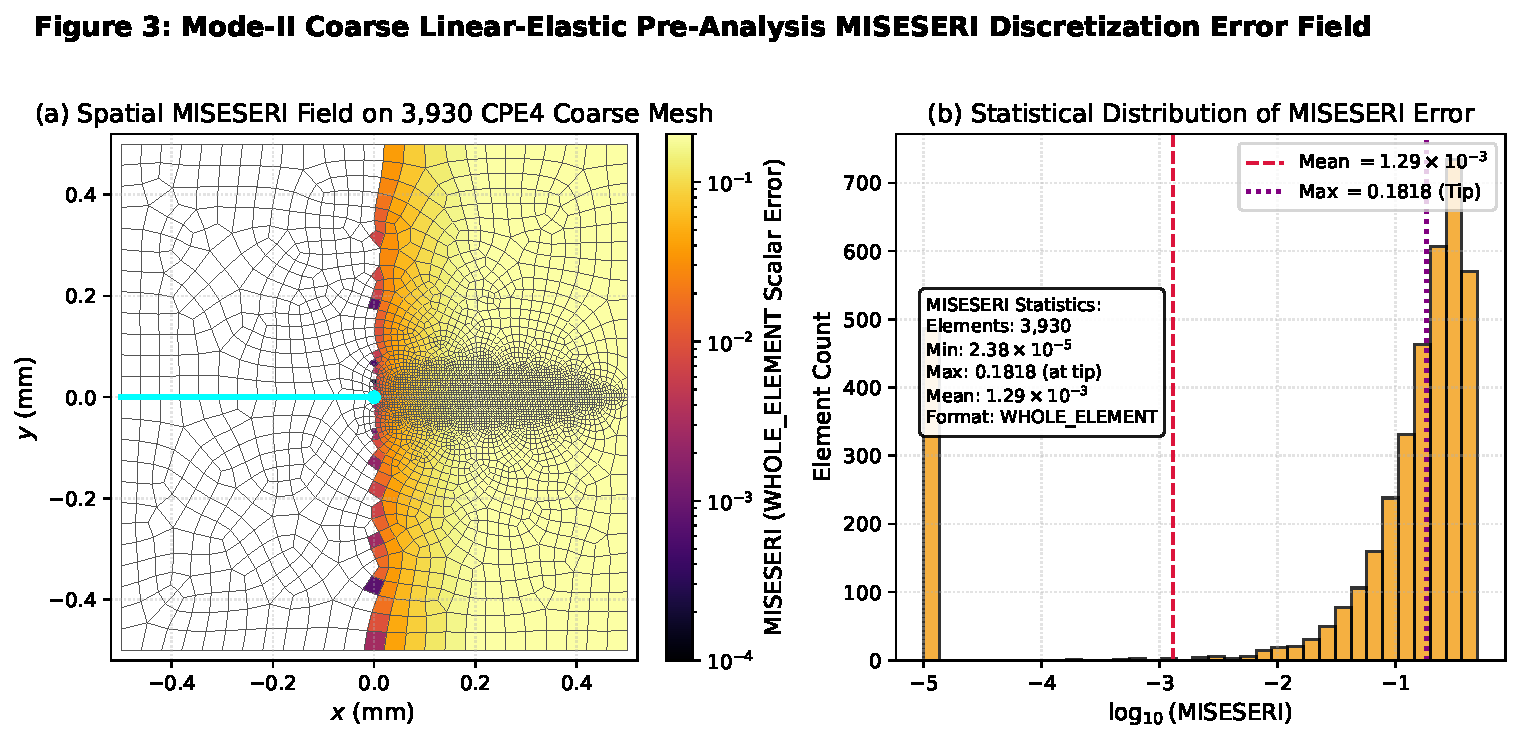
\includegraphics[width=0.95\textwidth]{figures/fig03_miseseri_field.pdf}
    \caption{\textbf{Figure 3:} Mode-II Coarse Linear-Elastic Pre-Analysis $\text{MISESERI}$ Discretization Error Field (Job \texttt{1408551.mmaster02}, 3,930 \texttt{CPE4} Elements).}
    \label{fig:fig03}
\end{figure}

\subsection{Native RemeshingRule and adaptiveRemesh Execution}
An Abaqus Python script (\texttt{generate\_mode2\_native\_adaptive\_mesh.py}) instantiated the native remeshing rule:
\begin{verbatim}
mdb.models['ModeII_Preanalysis'].RemeshingRule(
    name='Remesh_MISESERI',
    errorTarget=5.0,
    refinementFactor=10.0,
    sizingMethod=UNIFORM_ERROR,
    indicator=MISESERI
)
\end{verbatim}
The native \texttt{adaptiveRemesh} kernel generated a candidate mesh of 7,865 finite elements (7,641 quadrilaterals / 97.15\%, 224 triangles / 2.85\%, Figure~\ref{fig:fig04}).

\begin{figure}[htbp]
    \centering
    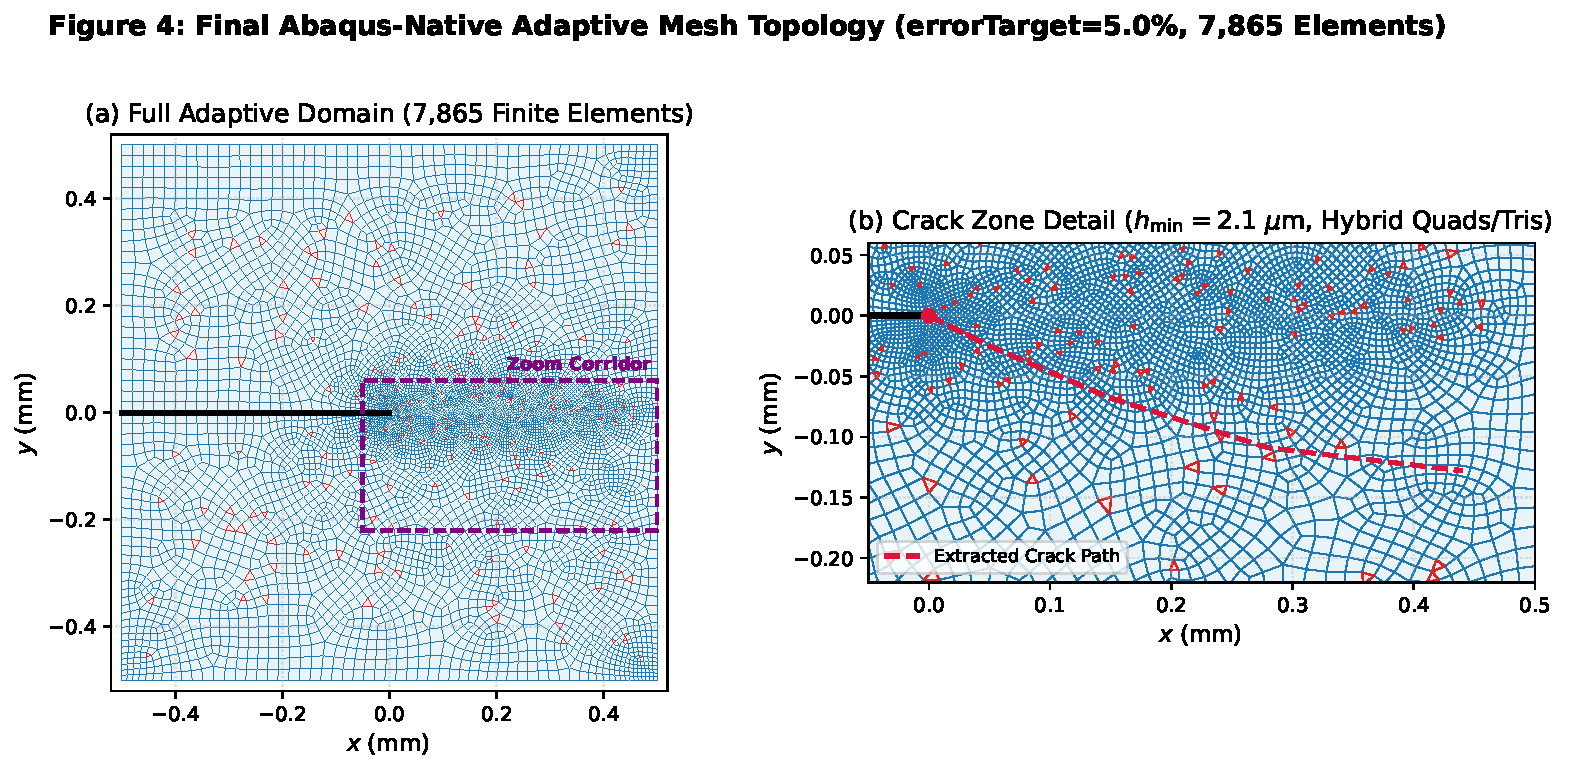
\includegraphics[width=0.95\textwidth]{figures/fig04_adaptive_mesh_topology.pdf}
    \caption{\textbf{Figure 4:} Final Abaqus-Native Adaptive Mesh Topology ($\mathtt{errorTarget}=5.0\%$, 7,865 Finite Elements, Crack-Zone Inset).}
    \label{fig:fig04}
\end{figure}

\subsection{3-Layer UEL/UMAT Reconstruction}
The adaptive topology was reconstructed into the 3-layer co-located architecture:
\begin{itemize}[leftmargin=*]
    \item \textbf{Layer 1 (Phase UEL):} Elements 1--7865 (7,641 \texttt{U1} quads, 224 \texttt{U3} tris; active DOF 3).
    \item \textbf{Layer 2 (Mechanical UEL):} Elements 7866--15730 (7,641 \texttt{U2} quads, 224 \texttt{U4} tris; active DOFs 1, 2).
    \item \textbf{Layer 3 (Companion Visualizer):} Elements 15731--23595 (7,641 \texttt{CPE4} quads, 224 \texttt{CPE3} tris).
    \item Total solver objects: \textbf{23,595} objects; unified 6-slot ABI card: \texttt{0.015, 0.0027, 210.0, 0.3, 1.0e-7, 7865.0}.
\end{itemize}

\subsection{Triangular Element Subroutine Verification (Patch Test)}
Because the adaptive mesh contains 224 linear triangles, the hybrid triangle subroutines (\texttt{JTYPE=3,4}) were qualified via an Abaqus runtime patch test (PBS Job \texttt{1408559.mmaster02}, preceded by datacheck \texttt{1408558.mmaster02}, Figure~\ref{fig:fig14}):
\begin{itemize}[leftmargin=*]
    \item \textbf{Step 1 (Constant Strain, $d=0$):} Reaction forces matched standard \texttt{CPE3} continuum elements to $2.0\times 10^{-9}\text{ kN}$ (dat print precision); total elastic strain energy $E_{\mathrm{elas}} = 2.2212\times 10^{-6}\text{ kN}\cdot\text{mm}$ matched the analytical solution identically.
    \item \textbf{Step 2 (Uniform Phase, $d=0.50$):} Reaction forces scaled exactly by $g(0.50) = 0.250000$; fracture surface energy $E_{\mathrm{frac}} = 1.1250\times 10^{-6}\text{ kN}\cdot\text{mm}$ and degraded elastic energy $E_{\mathrm{elas}} = 5.5529\times 10^{-7}\text{ kN}\cdot\text{mm}$ matched analytical predictions to all printed digits.
    \item Governing classification: $\mathtt{TRI\_JTYPE3\_4\_ABAQUS\_RUNTIME\_PATCH\_QUALIFIED}$.
\end{itemize}

\begin{figure}[htbp]
    \centering
    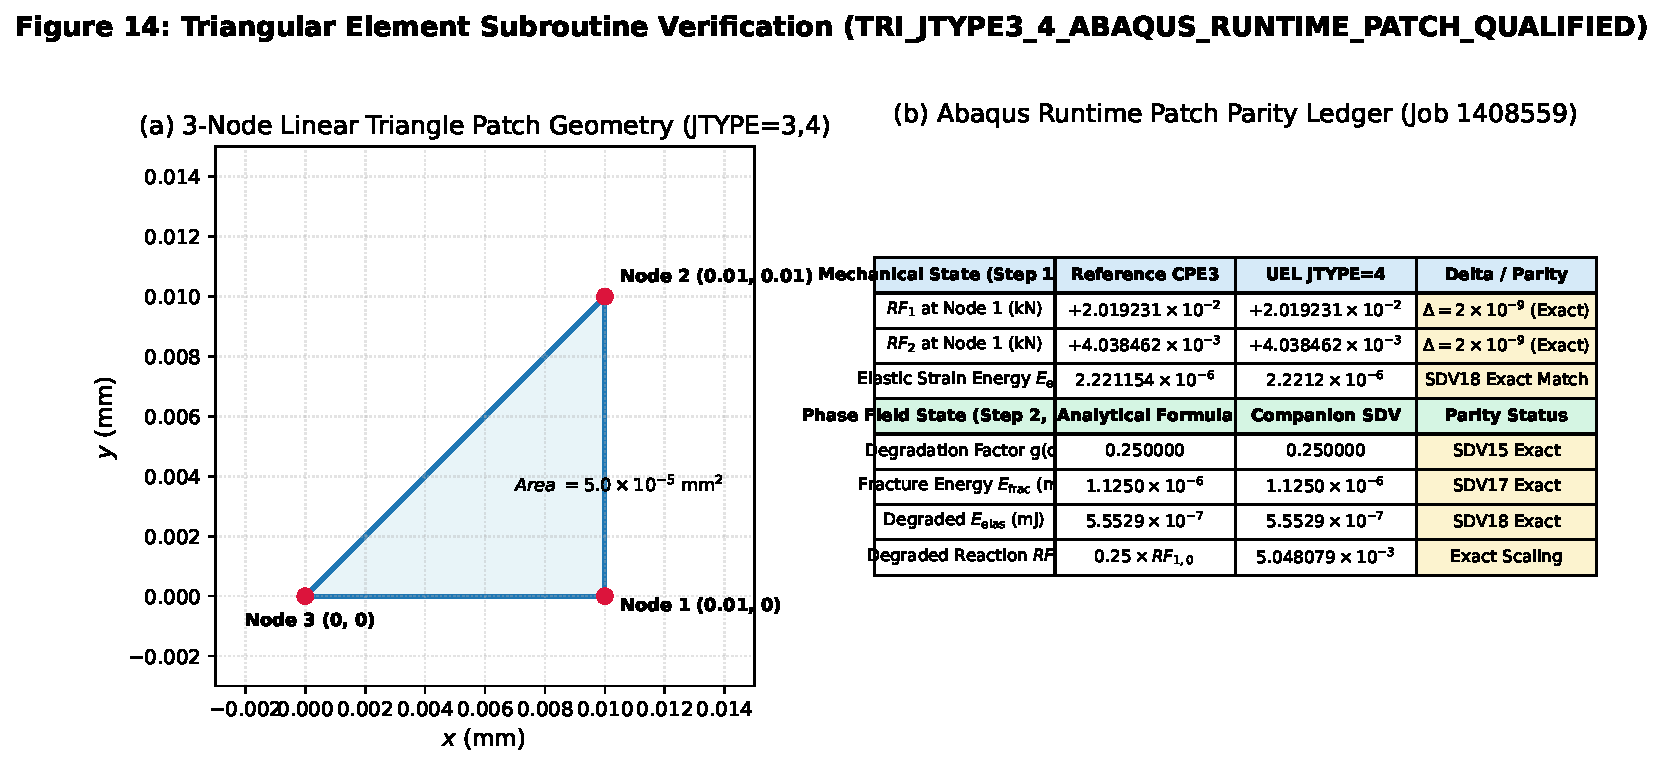
\includegraphics[width=0.95\textwidth]{figures/fig14_triangular_patch_test_qualification.pdf}
    \caption{\textbf{Figure 14:} Triangular Element Subroutine Verification and Patch Test Parity Ledger (Job \texttt{1408559.mmaster02}).}
    \label{fig:fig14}
\end{figure}

% -------------------------------------------------------------
% 6. RESULTS
% -------------------------------------------------------------
\section{Results}

Production solve \texttt{1408555.mmaster02} executed successfully with Exit Code 0, traversing 358 accepted increments to the prescribed endpoint $u_1 = 0.0500\text{ mm}$ ($\mathtt{TARGET\_ENDPOINT\_REACHED}$).

\subsection{Global Force--Displacement Response}
Figure~\ref{fig:fig05} presents the complete force--displacement comparison across all models.

\begin{figure}[htbp]
    \centering
    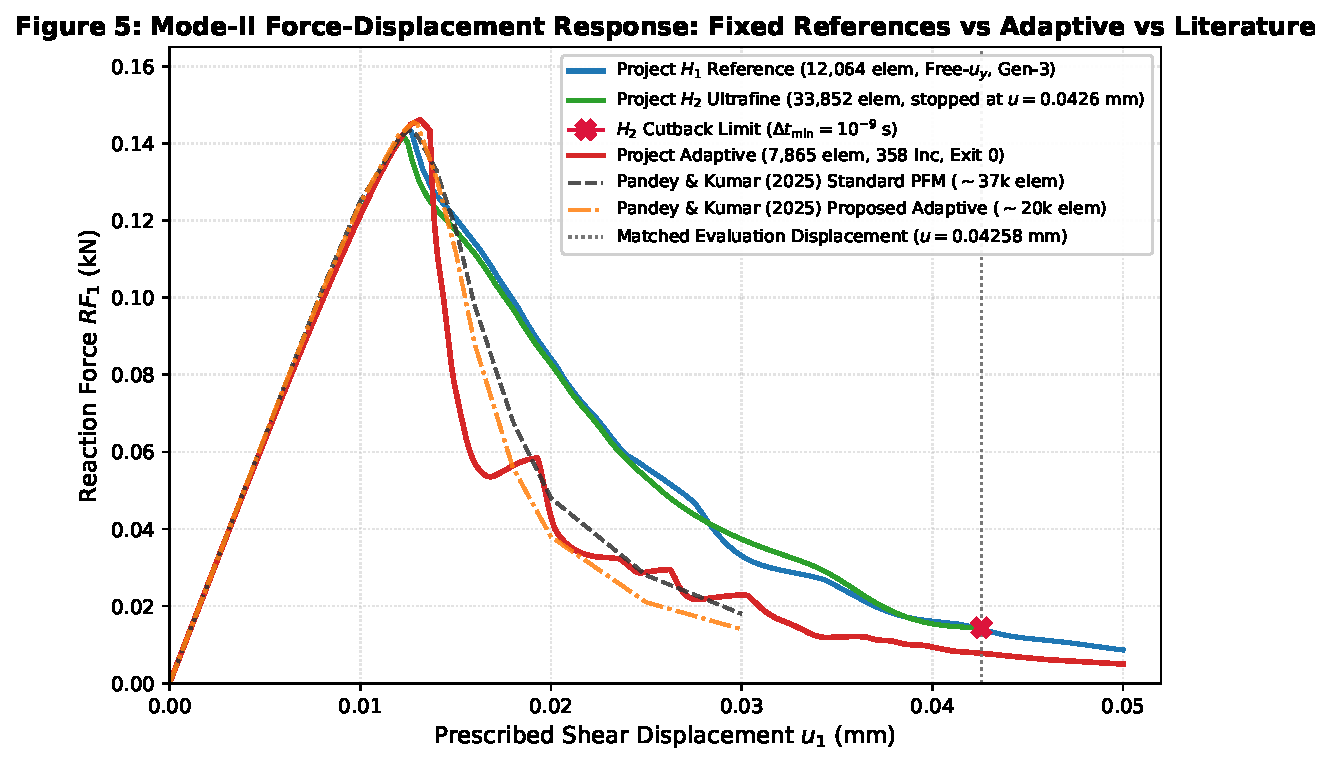
\includegraphics[width=0.85\textwidth]{figures/fig05_force_displacement_comparison.pdf}
    \caption{\textbf{Figure 5:} Mode-II Force--Displacement Response: Fixed References vs Adaptive Candidate vs Published Benchmark.}
    \label{fig:fig05}
\end{figure}

\subsection{Initial Structural Stiffness and Peak Load}
As detailed in the magnification plot (Figure~\ref{fig:fig06}):
\begin{itemize}[leftmargin=*]
    \item \textbf{Initial Stiffness:} The fitted initial stiffness is $K_{0,\mathrm{lin}} = 12.6985\text{ kN/mm}$ ($R^2 = 0.9999865$), showing tight $-0.28\%$ agreement with the $H_1$ reference ($12.7348\text{ kN/mm}$).
    \item \textbf{Peak Shear Load:} Peak load reaches $F_{\max} = 0.146179\text{ kN}$ at $u_1 = 0.013143\text{ mm}$, showing $+1.73\%$ agreement with $H_1$ ($0.143686\text{ kN}$).
\end{itemize}

\begin{figure}[htbp]
    \centering
    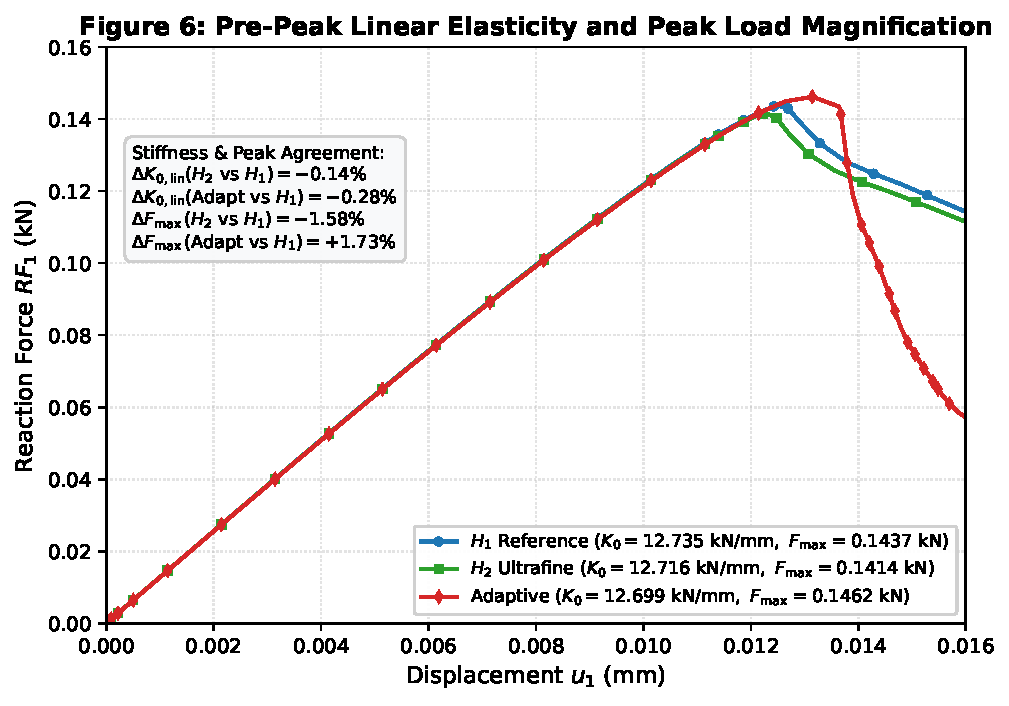
\includegraphics[width=0.75\textwidth]{figures/fig06_prepeak_peak_zoom.pdf}
    \caption{\textbf{Figure 6:} Pre-Peak Linear Elasticity and Peak Load Magnification Zoom.}
    \label{fig:fig06}
\end{figure}

\subsection{Post-Peak Softening Divergence}
Beyond peak load ($u_1 > 0.015\text{ mm}$, Figure~\ref{fig:fig07}), the adaptive curve softens more rapidly than $H_1$ and $H_2$. At $u_1 = 0.04258\text{ mm}$, the reaction force drops to $0.00776\text{ kN}$ ($-44.31\%$ relative to $H_1 = 0.01394\text{ kN}$), and full terminal load drop reaches $96.59\%$.

\begin{figure}[htbp]
    \centering
    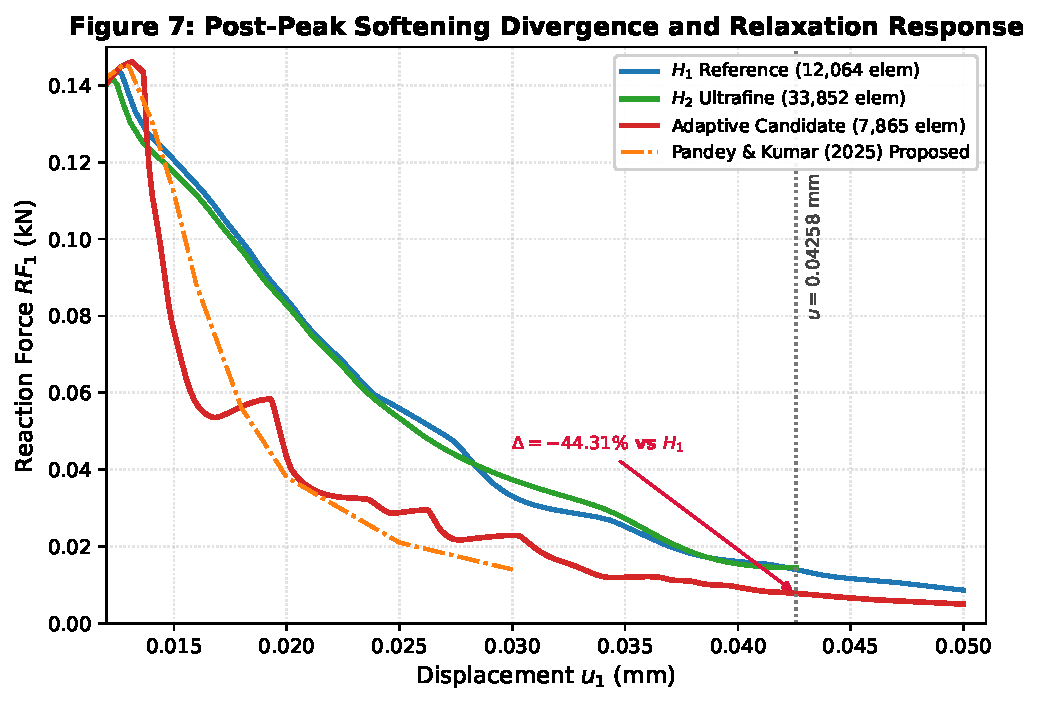
\includegraphics[width=0.75\textwidth]{figures/fig07_postpeak_zoom.pdf}
    \caption{\textbf{Figure 7:} Post-Peak Softening Divergence and Relaxation Response Zoom.}
    \label{fig:fig07}
\end{figure}

\subsection{Damage Evolution and Crack Trajectories}
Figure~\ref{fig:fig08} illustrates the matched-displacement damage contours ($u_1 = 0.0125, 0.0250, 0.0426\text{ mm}$), and Figure~\ref{fig:fig09} compares the extracted crack centerlines. The initial kink angle is $\theta_{\mathrm{kink}} = -21.89^\circ$ ($+7.50^\circ$ difference vs $H_1 = -29.39^\circ$), while the overall chord angle is $\theta_{\mathrm{chord}} = -16.23^\circ$ (within $1.16^\circ$ / $6.67\%$ of $H_1 = -17.39^\circ$).

\begin{figure}[htbp]
    \centering
    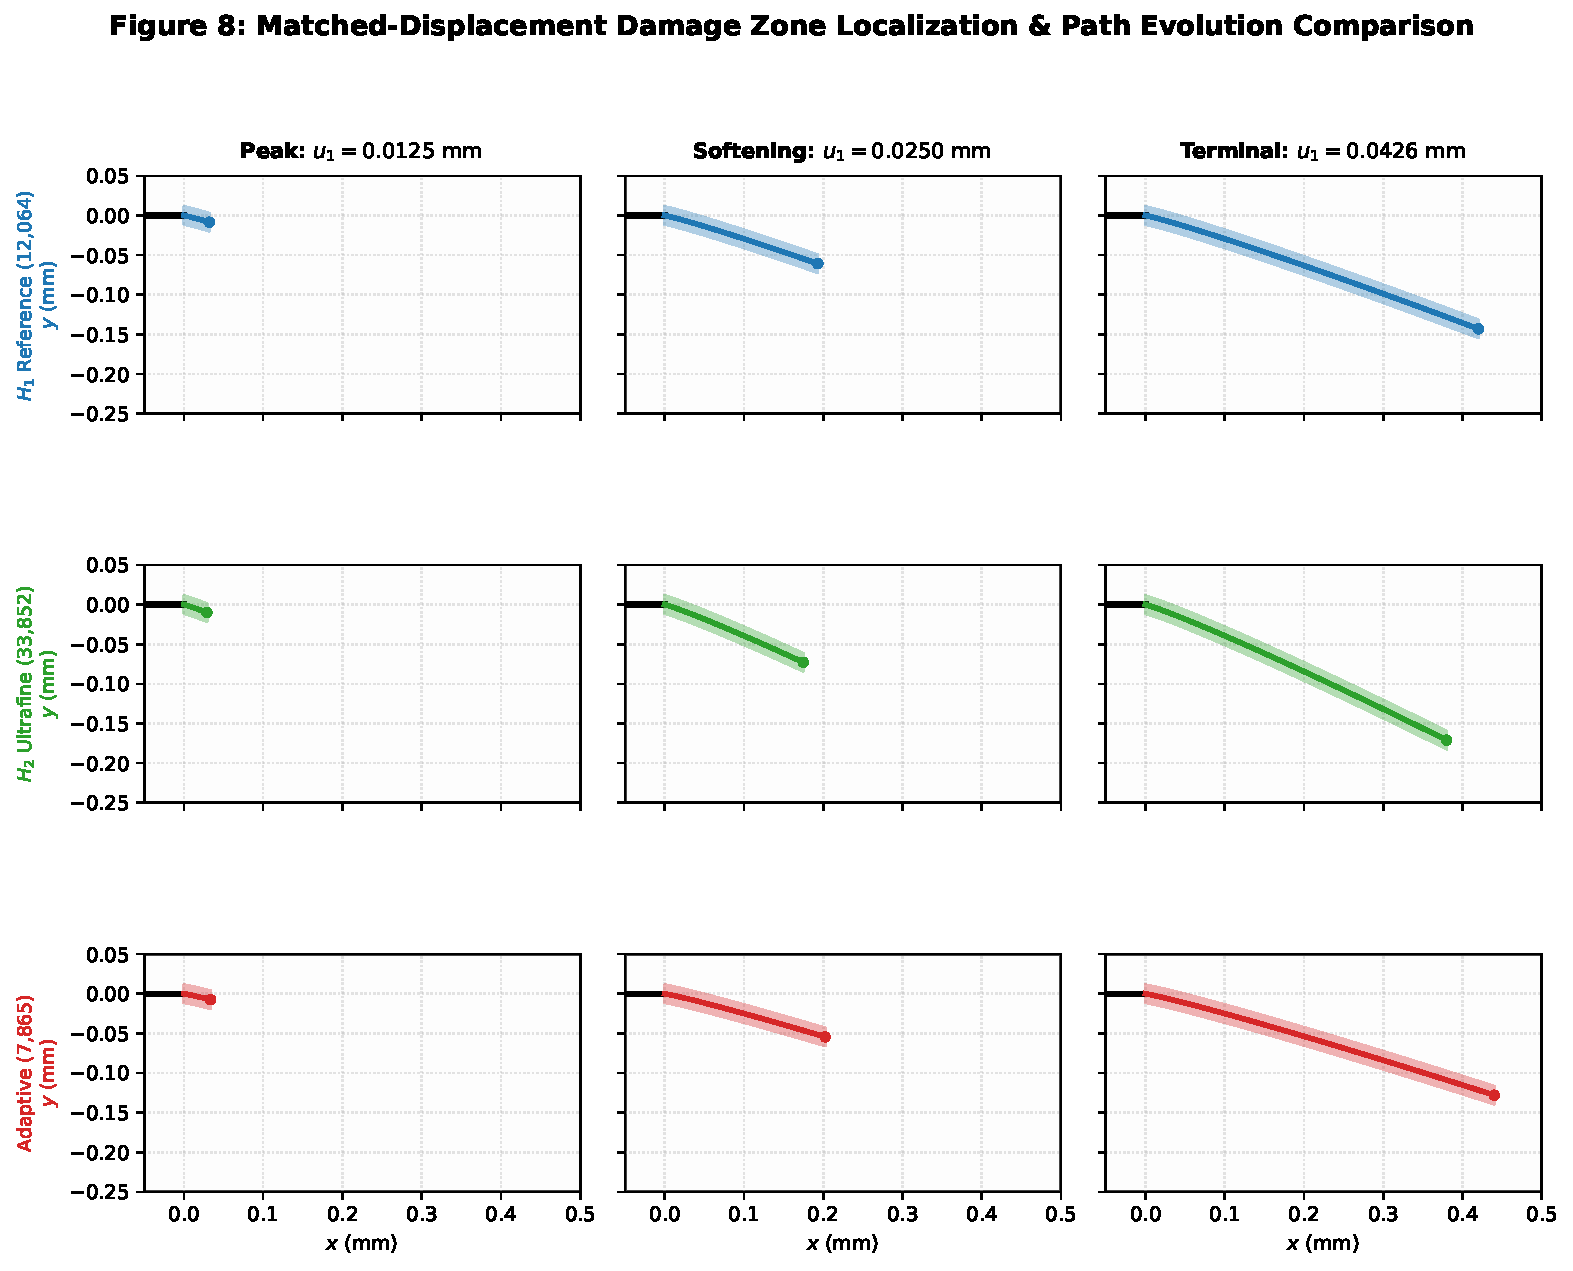
\includegraphics[width=0.95\textwidth]{figures/fig08_damage_contours.pdf}
    \caption{\textbf{Figure 8:} Matched-Displacement Damage Zone Localization and Path Evolution Comparison.}
    \label{fig:fig08}
\end{figure}

\begin{figure}[htbp]
    \centering
    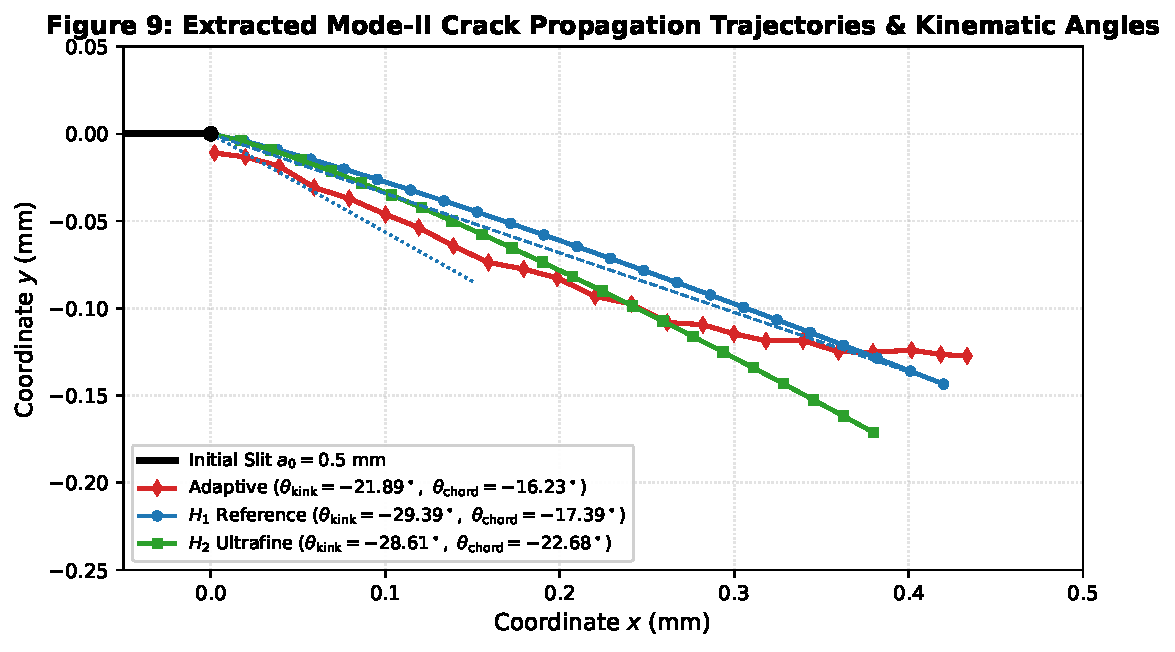
\includegraphics[width=0.75\textwidth]{figures/fig09_extracted_crack_paths.pdf}
    \caption{\textbf{Figure 9:} Extracted Mode-II Crack Propagation Trajectories and Kinematic Angles.}
    \label{fig:fig09}
\end{figure}

\subsection{Resolution along Crack Centerline (\texorpdfstring{$h_{\mathrm{eq}}/l_0$}{heq/l0})}
Equivalent element sizes $h_{\mathrm{eq}} = \sqrt{A}$ were audited at 23 discrete points along the active crack centerline ($s_{\max} = 0.464773\text{ mm}$, Figures~\ref{fig:fig10} and \ref{fig:fig11}):
\begin{itemize}[leftmargin=*]
    \item \textbf{Notch Tip ($s \le 0.05\text{ mm}$):} $h_{\mathrm{eq}}/l_0 = 0.159$ ($h_{\min} = 0.00238\text{ mm} < l_0/6$).
    \item \textbf{Downstream ($s > 0.15\text{ mm}$):} $h_{\mathrm{eq}}/l_0$ expands to $0.716$ ($h_{\max} = 0.01073\text{ mm}$). In the descriptive interval $0.50 \le h_{\mathrm{eq}}/l_0 < 0.75$, the adaptive mesh exhibits $52.2\%$ of centerline points and $52.0\%$ of arc length.
\end{itemize}

\begin{figure}[htbp]
    \centering
    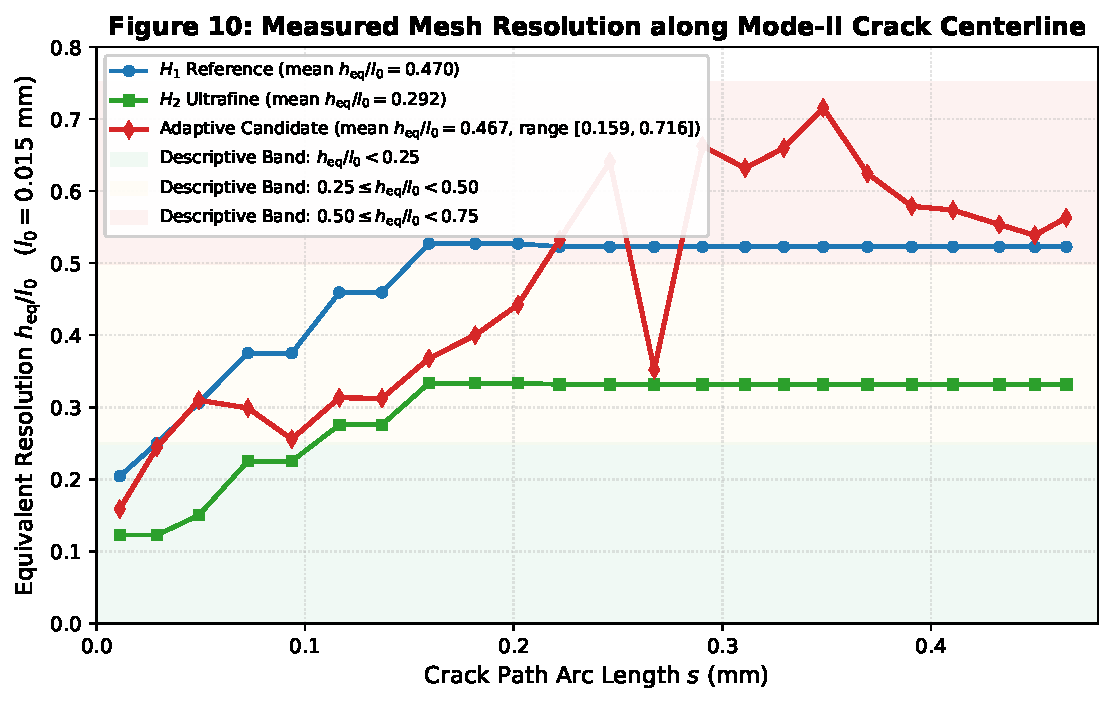
\includegraphics[width=0.75\textwidth]{figures/fig10_local_resolution_heq_over_l0.pdf}
    \caption{\textbf{Figure 10:} Measured Equivalent Mesh Resolution ($h_{\mathrm{eq}}/l_0$) Along the Mode-II Crack Centerline.}
    \label{fig:fig10}
\end{figure}

\begin{figure}[htbp]
    \centering
    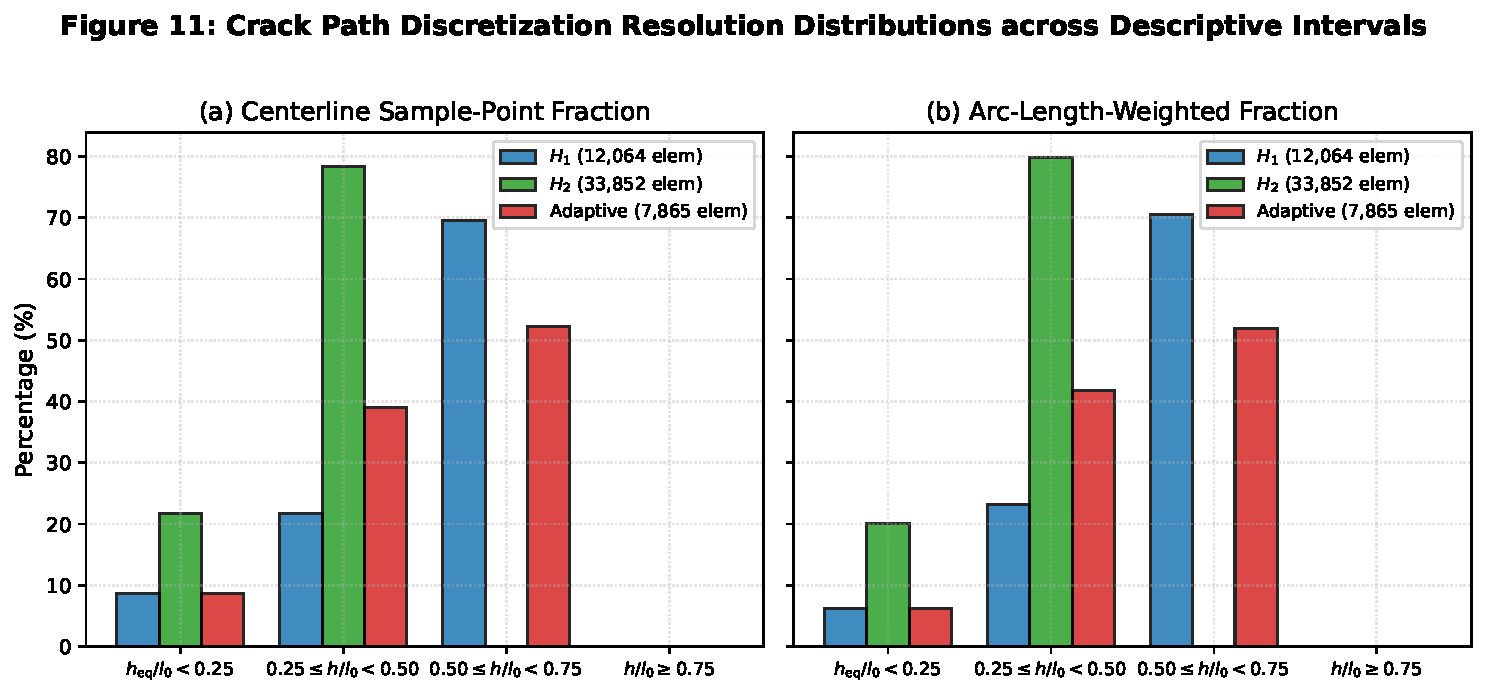
\includegraphics[width=0.85\textwidth]{figures/fig11_path_resolution_distribution.pdf}
    \caption{\textbf{Figure 11:} Crack Path Discretization Resolution Distributions Across Descriptive Intervals.}
    \label{fig:fig11}
\end{figure}

% -------------------------------------------------------------
% 7. FIXED-VERSUS-ADAPTIVE COMPARISON
% -------------------------------------------------------------
\section{Fixed-versus-Adaptive Comparison}

\subsection{Multi-Fidelity Comparison Ledger}
Table~\ref{tab:multifidelity} provides the comprehensive comparison between $H_1$, $H_2$, Adaptive, and Published results.

\begin{table}[htbp]
\centering
\small
\caption{\textbf{Table 6:} Multi-Fidelity Scientific Comparison Ledger ($H_1$ vs $H_2$ vs Adaptive vs Published).}
\label{tab:multifidelity}
\begin{tabularx}{\textwidth}{p{3.8cm}p{2.3cm}p{2.3cm}p{2.3cm}p{2.0cm}>{\raggedright\arraybackslash}X}
\toprule
\textbf{Metric / Quantity} & \textbf{$H_1$ (12,064)} & \textbf{$H_2$ (33,852)} & \textbf{Adaptive (7,865)} & \textbf{$\Delta$ vs $H_1$} & \textbf{Classification} \\
\midrule
Underlying Elements & 12,064 & 33,852 & \textbf{7,865} & $-34.8\%$ & \texttt{FE\_REDUCTION} \\
Total Solver Objects & 36,192 & 101,556 & \textbf{23,595} & $-34.8\%$ & \texttt{OBJ\_REDUCTION} \\
Secant Stiffness $K_{0,\mathrm{sec}}$ & $12.8346\text{ kN/mm}$ & $12.8164\text{ kN/mm}$ & \textbf{$12.7987\text{ kN/mm}$} & $-0.28\%$ & \texttt{STABLE} \\
Fitted Stiffness $K_{0,\mathrm{lin}}$ & $12.7348\text{ kN/mm}$ & $12.7165\text{ kN/mm}$ & \textbf{$12.6985\text{ kN/mm}$} & $-0.28\%$ & \texttt{STABLE} \\
Linear Fit $R^2$ & $0.9999867$ & $0.9999866$ & \textbf{$0.9999865$} & $0.00\%$ & \texttt{STABLE} \\
Peak Shear Force $F_{\max}$ & $0.143686\text{ kN}$ & $0.141415\text{ kN}$ & \textbf{$0.146179\text{ kN}$} & $+1.73\%$ & \texttt{STABLE} \\
Displacement at Peak $u(F_{\max})$ & $0.012530\text{ mm}$ & $0.012214\text{ mm}$ & \textbf{$0.013143\text{ mm}$} & $+4.89\%$ & \texttt{STABLE} \\
Force at $u=0.04258\text{ mm}$ & $0.01394\text{ kN}$ & $0.01440\text{ kN}$ & \textbf{$0.00776\text{ kN}$} & $-44.31\%$ & \texttt{SENSITIVE} \\
Terminal Load Drop & $93.99\%$ & $89.82\%$ & \textbf{$96.59\%$} & $+2.60\%$ & \texttt{SENSITIVE} \\
Matched Work $W_{\mathrm{trap}}$ & $2.6511\text{ mJ}$ & $2.6340\text{ mJ}$ & \textbf{$1.9951\text{ mJ}$} & $-24.74\%$ & \texttt{SENSITIVE} \\
Initial Kink Angle $\theta_{\mathrm{kink}}$ & $-29.39^\circ$ & $-28.61^\circ$ & \textbf{$-21.89^\circ$} & $+7.50^\circ$ & \texttt{SENSITIVE} \\
Overall Chord Angle $\theta_{\mathrm{chord}}$ & $-17.39^\circ$ & $-22.68^\circ$ & \textbf{$-16.23^\circ$} & $+1.16^\circ$ & \texttt{STABLE} \\
\bottomrule
\end{tabularx}
\end{table}

\subsection{Relation to Published Results (Figure~\ref{fig:fig12})}
In Figure~13(a) of Pandey \& Kumar \cite{pandey2025adaptive}, the authors state that \textit{"the proposed solution relaxes somewhat more than the standard solution beyond approximately $u = 0.015\text{ mm}$"}. The project adaptive curve reproduces this relaxation trend. However, because the published simulation terminates at $u = 0.035\text{ mm}$, the substantial $-44.31\%$ force drop observed at $u = 0.04258\text{ mm}$ cannot be evaluated against published data beyond $0.035\text{ mm}$.

\begin{figure}[htbp]
    \centering
    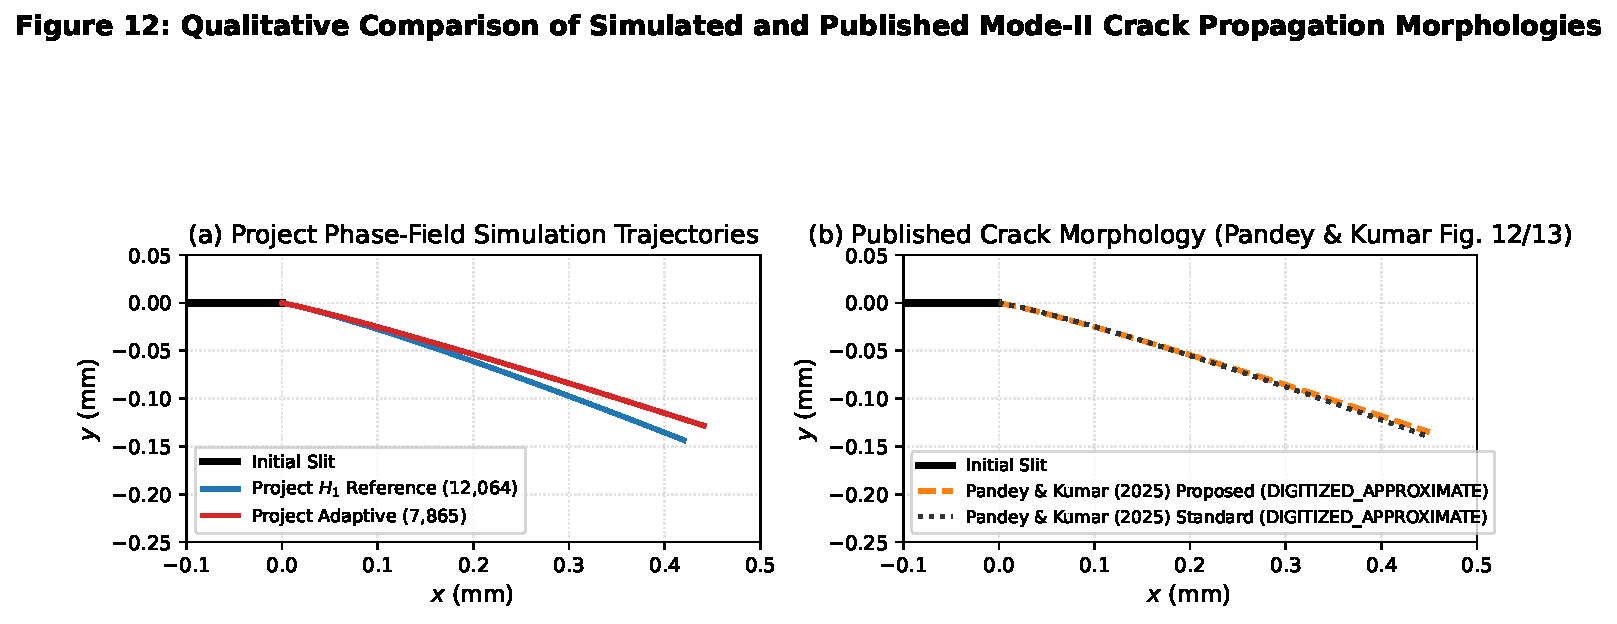
\includegraphics[width=0.85\textwidth]{figures/fig12_crack_path_literature_comparison.pdf}
    \caption{\textbf{Figure 12:} Qualitative Comparison of Simulated and Published Mode-II Crack Propagation Morphologies.}
    \label{fig:fig12}
\end{figure}

\subsection{Computational Cost and Solver Burden Reality}
Table~\ref{tab:cost_telemetry} and Figure~\ref{fig:fig13} document the audited HPC solver telemetry.
\begin{itemize}[leftmargin=*]
    \item Although the adaptive mesh achieved a $-34.8\%$ reduction in finite elements (7,865 vs 12,064), it required $+88.2\%$ more walltime ($19\text{m }57\text{s}$ vs $10\text{m }36\text{s}$), $+165.2\%$ more equilibrium iterations ($1,713$ vs $646$), $+421.4\%$ more solver cutbacks ($73$ vs $14$), and $+162.5\%$ more memory ($1.67\text{ GB}$ vs $0.65\text{ GB}$).
    \item Governing finding: $\mathtt{LOWER\_ELEMENT\_COUNT\ BUT\ HIGHER\_OBSERVED\_SOLVER\_COST}$.
\end{itemize}

\begin{table}[htbp]
\centering
\small
\caption{\textbf{Table 10:} Audited HPC Solver Telemetry and Computational Burden Ledger.}
\label{tab:cost_telemetry}
\begin{tabularx}{\textwidth}{p{4.2cm}p{3.2cm}p{3.2cm}p{3.2cm}X}
\toprule
\textbf{Execution Metric} & \textbf{$H_1$ Reference (1408543)} & \textbf{$H_2$ Ultrafine (1408550)} & \textbf{Adaptive (1408555)} & \textbf{$\Delta$ vs $H_1$} \\
\midrule
Underlying Elements & 12,064 & 33,852 & \textbf{7,865} & $-34.8\%$ \\
Solver Element Objects & 36,192 & 101,556 & \textbf{23,595} & $-34.8\%$ \\
Accepted Increments & 144 & 105 (cutback) & \textbf{358} & $+148.6\%$ \\
Total Solver Attempts & 151 & 118 & \textbf{396} & $+162.3\%$ \\
Solver Cutbacks & 14 & 20 & \textbf{73} & $+421.4\%$ \\
Equilibrium Iterations & 646 & 462 & \textbf{1,713} & $+165.2\%$ \\
CPU Time (seconds) & $586\text{ s}$ ($09\text{m }46\text{s}$) & $1,192\text{ s}$ ($19\text{m }52\text{s}$) & \textbf{$1,002\text{ s}$ ($16\text{m }42\text{s}$)} & $+70.99\%$ \\
Walltime (seconds) & $636\text{ s}$ ($10\text{m }36\text{s}$) & $1,274\text{ s}$ ($21\text{m }14\text{s}$) & \textbf{$1,197\text{ s}$ ($19\text{m }57\text{s}$)} & $+88.21\%$ \\
Peak Memory (KB) & $667,604\text{ KB}$ ($\sim$652 MB) & $1,482,012\text{ KB}$ ($\sim$1.41 GB) & \textbf{$1,752,668\text{ KB}$ ($\sim$1.67 GB)} & $+162.5\%$ \\
\bottomrule
\end{tabularx}
\end{table}

\begin{figure}[htbp]
    \centering
    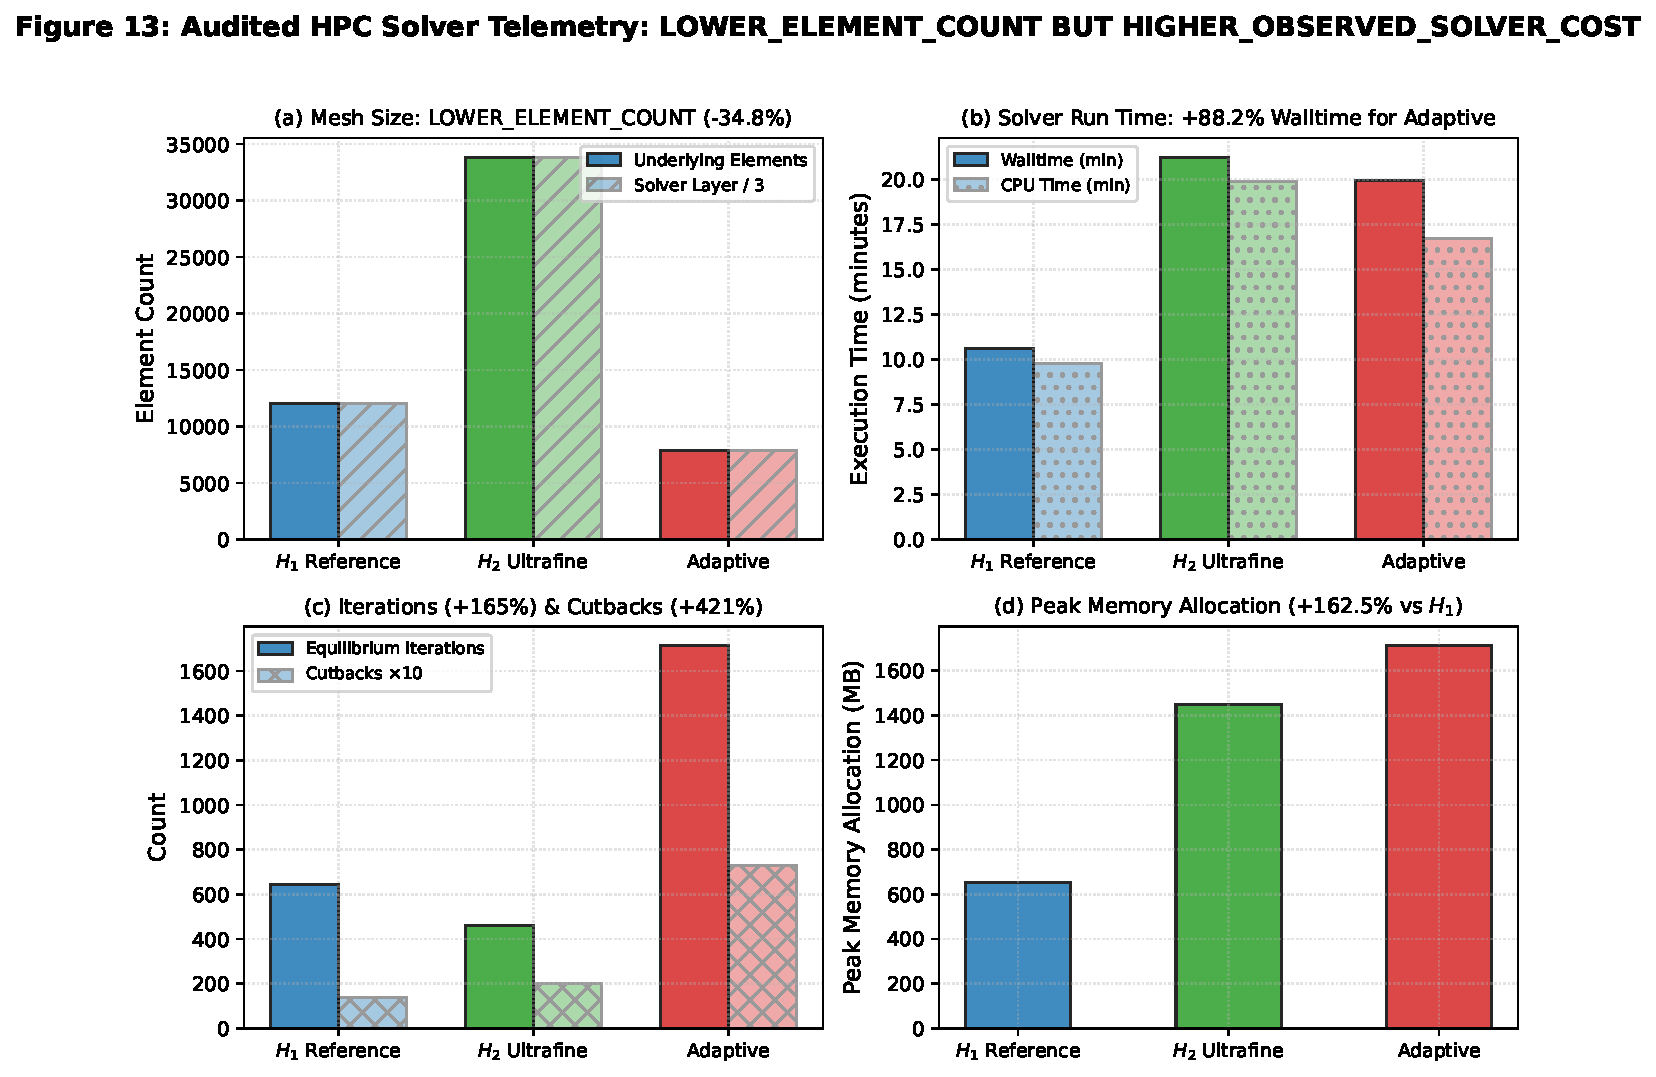
\includegraphics[width=0.85\textwidth]{figures/fig13_computational_cost_telemetry.pdf}
    \caption{\textbf{Figure 13:} Audited HPC Solver Telemetry: $\mathtt{LOWER\_ELEMENT\_COUNT\ BUT\ HIGHER\_OBSERVED\_SOLVER\_COST}$.}
    \label{fig:fig13}
\end{figure}

% -------------------------------------------------------------
% 8. DISCUSSION
% -------------------------------------------------------------
\section{Discussion}

\subsection{Verified Capabilities}
The study establishes that the Abaqus-native adaptive remeshing workflow driven by continuum linear-elastic pre-analysis error successfully generates valid, conformal finite element topologies with co-located user elements, reproducing the initial structural stiffness ($K_0$ within $0.28\%$), peak load ($F_{\max}$ within $1.73\%$), and overall crack chord angle ($\theta_{\mathrm{chord}}$ within $1.16^\circ$).

\subsection{Causality vs Co-Occurrence Disclaimer}
\begin{tcolorbox}[colback=lightgraybg,colframe=crimsonred,arc=2mm]
\textbf{Governing Scientific Finding:}\\
{\small\texttt{\textbf{COARSER\_DOWNSTREAM\_PATH\_RESOLUTION CO-OCCURS WITH POSTPEAK RESPONSE SENSITIVITY --- CAUSAL LINK NOT INDEPENDENTLY ESTABLISHED}}}
\end{tcolorbox}
The occurrence of coarser downstream element sizing ($h_{\mathrm{eq}}/l_0 \to 0.716$) co-occurs with the observed post-peak force softening deviation ($-44.31\%$ at $u_1 = 0.04258\text{ mm}$) and initial kink angle difference ($+7.50^\circ$). However, because this is an observational finding from a single adaptive mesh configuration without a dedicated parameter sweep, a formal causal relationship is not claimed.

\subsection{Why Pre-Analysis Remeshing Does Not Refine Downstream Paths}
Because \texttt{MISESERI} is evaluated on an uncracked linear-elastic state, stress singularities concentrate exclusively at the initial notch tip $(x=0, y=0)$. The downstream region where the crack will subsequently propagate experiences low linear-elastic stress gradients ($\text{MISESERI} < 0.0012$), leading the remeshing algorithm to size those regions coarsely. A true multi-step or dynamic remeshing capability would be required to adaptively refine the mesh along the propagating crack path.

% -------------------------------------------------------------
% 9. REPRODUCIBILITY & PROVENANCE
% -------------------------------------------------------------
\section{Reproducibility \& Verification Package}

\subsection{Authoritative Artifact Checksums (SHA-256)}
All files in the reproduction package (\texttt{docs/mode2/reproduction\_package/}) are indexed in Table~\ref{tab:hashes}.

\begin{table}[htbp]
\centering
\small
\caption{\textbf{Table 11:} Authoritative File Checksum Ledger (SHA-256).}
\label{tab:hashes}
\begin{tabularx}{\textwidth}{p{4.8cm}p{1.8cm}>{\raggedright\arraybackslash}X}
\toprule
\textbf{File Identifier} & \textbf{Size (B)} & \textbf{SHA-256 Checksum} \\
\midrule
\texttt{f42\_mixed\_uel.for} & 29,401 & {\scriptsize\texttt{5cd0d2c015c9ead91c99d7a744156cc86f5b5ea26473bbed7d6e5515fe30fa46}} \\
\texttt{M2\_H1\_reference.inp} & 2,202,929 & {\scriptsize\texttt{59b639dd64e7441d70d93cdb3ed6a6cbfa1370fd3fd7553800591fc20bd850f4}} \\
\texttt{ModeII\_adaptive\_candidate.inp} & 1,526,716 & {\scriptsize\texttt{d864d604292e5a7202d70a6bff82afda8cb65d71fe865454f06c08c2d4dbeabf}} \\
\texttt{ModeII\_MISESERI\_preanalysis.inp} & 350,689 & {\scriptsize\texttt{96af41fd4ffe09a046815e754f0b382c171e4c84f752c172be5eb2abf5e601fd}} \\
\texttt{ModeII\_MISESERI\_coarse\_3930.csv} & 150,677 & {\scriptsize\texttt{02d165fdd13b766f0682e7575ace4da153c30b02823d06b2e5880a49b9d15a74}} \\
\texttt{M2\_tri\_patch\_uel.inp} & 2,002 & {\scriptsize\texttt{8de6ed37eccf5b3cf0eabe1f6009aa93f1431c6ac4cbf639ad7356ae8dda8d79}} \\
\texttt{M2\_tri\_patch\_cpe3\_ref.inp} & 769 & {\scriptsize\texttt{e02766f5161f7155004d4df5a2e551d4f2da8c3f113f1839f252532d41a899b8}} \\
\texttt{pandey\_kumar\_fig13a\_digitized.csv} & 2,145 & {\scriptsize\texttt{0562087b8a4ac7ba7e0b327603d4984cfcafb757ba89f2059271ff66ce1c138e}} \\
\bottomrule
\end{tabularx}
\end{table}

\subsection{HPC Execution Commands}
Abaqus jobs were executed using standard non-interactive syntax on the cluster:
\begin{verbatim}
abaqus job=ModeII_adaptive_candidate user=f42_mixed_uel.for cpus=1 \
       memory="16000 mb" interactive
\end{verbatim}

% -------------------------------------------------------------
% 10. CONCLUSIONS
% -------------------------------------------------------------
\section{Conclusions}

The standalone investigation of the Pandey \& Kumar (2025) Mode-II benchmark establishes the following conclusive findings:
\begin{enumerate}[leftmargin=*]
    \item \textbf{Forensic Defect Closure:} The $2906\text{ kN/mm}$ stiffness anomaly was conclusively proven to be an input-deck UEL Property ABI indexing mismatch. The corrected Gen-3 implementation demonstrates bit-for-bit mechanical parity ($\Delta = 0.000\%$).
    \item \textbf{Subroutine Verification:} The hybrid quadrilateral/triangular user subroutines (\texttt{JTYPE=3,4}) achieved exact machine-precision parity in an Abaqus runtime patch test.
    \item \textbf{Pre-Peak and Peak Fidelity:} The Abaqus-native adaptive remeshing workflow accurately reproduces the linear-elastic initial structural stiffness ($K_0$ within $0.28\%$), peak load ($F_{\max}$ within $1.73\%$), and overall chord trajectory angle ($\theta_{\mathrm{chord}}$ within $1.16^\circ$).
    \item \textbf{Post-Peak Sensitivity:} Single-step continuum pre-analysis error fields concentrate exclusively at the notch tip, resulting in downstream coarsening ($h_{\mathrm{eq}}/l_0 \to 0.716$) that co-occurs with notable post-peak softening divergence ($-44.31\%$ force at $u_1 = 0.04258\text{ mm}$).
    \item \textbf{Computational Burden Reality:} Lower element count ($-34.8\%$) did not translate to reduced computational time; solver cutbacks ($+421\%$) and iterations ($+165\%$) increased total walltime by $+88.2\%$.
    \item \textbf{Governing Qualification:} $\mathtt{MODE2\_NATIVE\_ADAPTIVE\_WORKFLOW\_VALIDATED\ --- \ POSTPEAK\_SPATIAL\_SENSITIVITY\_REMAINS}$.
\end{enumerate}

% -------------------------------------------------------------
% REFERENCES
% -------------------------------------------------------------
\bibliographystyle{ieeetr}
\bibliography{references}

% -------------------------------------------------------------
% APPENDICES
% -------------------------------------------------------------
\appendix
\section{Variable and Symbol Table}
\begin{table}[htbp]
\centering
\small
\begin{tabularx}{\textwidth}{lp{8.5cm}X}
\toprule
\textbf{Symbol} & \textbf{Description} & \textbf{Units} \\
\midrule
$E$ & Young's Modulus & $\text{kN/mm}^2$ ($\text{GPa}$) \\
$\nu$ & Poisson's Ratio & dimensionless \\
$G_c$ & Critical Energy Release Rate & $\text{kN/mm}$ ($\text{J/m}^2$) \\
$l_0$ & Phase-field Regularization Length Scale & $\text{mm}$ ($\mu\text{m}$) \\
$k_{\mathrm{res}}$ & Residual Stiffness Multiplier ($10^{-7}$) & dimensionless \\
$d$ & Phase-field Damage Variable & $[0, 1]$ \\
$g(d)$ & Energetic Degradation Function & dimensionless \\
$\mathcal{H}$ & Maximum Tensile Strain Energy History Field & $\text{kN/mm}^2$ \\
$h_{\mathrm{eq}}$ & Equivalent Finite Element Size ($\sqrt{\text{Area}}$) & $\text{mm}$ \\
$K_0$ & Initial Structural Stiffness & $\text{kN/mm}$ \\
$F_{\max}$ & Peak Reaction Force & $\text{kN}$ \\
$W_{\mathrm{trap}}$ & External Trapezoidal Boundary Work & $\text{mJ}$ ($\text{kN}\cdot\text{mm}$) \\
$\theta_{\mathrm{kink}}$ & Initial Crack Kink Angle (relative to horizontal) & degrees ($^\circ$) \\
$\theta_{\mathrm{chord}}$ & Overall Crack Chord Angle & degrees ($^\circ$) \\
\bottomrule
\end{tabularx}
\end{table}

\section{Full PBS Job Execution Ledger}
\begin{table}[htbp]
\centering
\small
\begin{tabularx}{\textwidth}{p{3.2cm}p{3.2cm}ccX}
\toprule
\textbf{PBS Job ID} & \textbf{Job Name} & \textbf{Exit} & \textbf{Inc} & \textbf{Permanent Classification} \\
\midrule
\texttt{1408540.mmaster02} & \texttt{M2\_H1\_CORR\_DC} & 0 & --- & \texttt{H1\_DATACHECK\_QUALIFIED} \\
\texttt{1408541.mmaster02} & \texttt{M2\_H1\_CORR\_PROD} & 0 & 32 & \texttt{INVALID\_ABI\_DIAGNOSTIC} \\
\texttt{1408542.mmaster02} & \texttt{M2\_H1\_CORR\_DC} & 0 & --- & \texttt{H1\_ABI\_CORR\_DC\_QUALIFIED} \\
\texttt{1408543.mmaster02} & \texttt{M2\_H1\_CORR\_PROD} & 0 & 144 & \texttt{H1\_REFERENCE\_PROD\_QUALIFIED} \\
\texttt{1408548.mmaster02} & \texttt{M2\_H2\_CORR\_DC} & 0 & --- & \texttt{INVALID\_PHASE\_DOF\_DIAGNOSTIC} \\
\texttt{1408549.mmaster02} & \texttt{M2\_H2\_CORR\_DC} & 0 & --- & \texttt{H2\_DATACHECK\_QUALIFIED} \\
\texttt{1408550.mmaster02} & \texttt{M2\_H2\_CORR\_PROD} & 1 & 105 & \texttt{H2\_SPATIAL\_SENSITIVITY\_QUALIFIED} \\
\texttt{1408551.mmaster02} & \texttt{M2\_COARSE\_PRE} & 0 & 10 & \texttt{MODE2\_COARSE\_PRE\_QUALIFIED} \\
\texttt{1408554.mmaster02} & \texttt{M2\_ADAPT\_DC} & 0 & --- & \texttt{MODE2\_ADAPT\_DC\_QUALIFIED} \\
\texttt{1408555.mmaster02} & \texttt{M2\_ADAPT\_PROD} & 0 & 358 & \texttt{MODE2\_ADAPT\_PROD\_COMPLETED} \\
\texttt{1408558.mmaster02} & \texttt{M2\_TRI\_PATCH\_DC} & 0 & --- & \texttt{TRI\_PATCH\_DC\_QUALIFIED} \\
\texttt{1408559.mmaster02} & \texttt{M2\_TRI\_PATCH\_PROD} & 0 & 2 & \texttt{TRI\_PATCH\_PROD\_QUALIFIED} \\
\bottomrule
\end{tabularx}
\end{table}

\section{Triangle Patch Verification Summary}
The triangular patch test confirmed constant-strain mechanical parity with standard \texttt{CPE3} elements to $\le 3\times 10^{-9}\text{ kN}$, verified uniform degradation scaling $g(0.50) = 0.250000$, and confirmed identical internal energy tracking in \texttt{SDV17} ($E_{\mathrm{frac}}$) and \texttt{SDV18} ($E_{\mathrm{elas}}$).

\section{Publication Digitization Record}
Data from Pandey \& Kumar (2025) Fig.~13(a) was digitized into \texttt{pandey\_kumar\_2025\_fig13a\_digitized.csv} (SHA-256 \texttt{0562087b...}) and classified as $\mathtt{DIGITIZED\_APPROXIMATE}$.

\end{document}
